\documentclass[12pt]{article}

\usepackage{graphicx}
\usepackage{caption}
\usepackage{amsfonts}
\usepackage{amsmath}
\usepackage{xcolor}
\usepackage{subfig}
\usepackage{subfloat}
\usepackage{hyperref}
\usepackage{eurosym}
\usepackage{xcolor,colortbl} % Color en tablas
\definecolor{LightGrey}{rgb}{0.85,0.85,0.85}
\usepackage[a4paper]{geometry}                                
\usepackage{enumitem}    

\newcommand{\degree}{^{\circ}C}

\newcommand{\LinkColor}{blue}	% Link color
\hypersetup{
		{colorlinks},
		{linkcolor=\LinkColor},
		{citecolor=\LinkColor},
		{urlcolor=\LinkColor},
}
\usepackage[
%	language = spanish,
	url = true,
	%style = authoryear,
	hyperref = true,
	backref = true,
	backend = biber,
	sorting = none,
	]{biblatex}
	
\bibliography{References}

\graphicspath{{IMG/}{IMG/Results/}}
	
\begin{document}
    \raggedbottom
    \sloppy \lefthyphenmin=1000
    \setlength{\parskip}{3ex}

\title{NEW Tracking Plane Subproject \\Status Report (May 2016)}

\author{J. Rodr\'iguez, M. Querol, A. Mart\'inez, S. C\'arcel, A. Sim\'on, F. Monrabal, \\ J. Toledo, J.J. G\'omez-Cadenas}
\date{May-2016}

\maketitle

\section*{Abstract}

This work describes the tracking plane of the NEW detector, including the sensors, front-end electronics, cables, custom feedthroughs and power supply. 
\clearpage

\tableofcontents

\clearpage


\section{New kapton Dice-Boards}
The NEW tracking plane is (TP) permits the reconstruction of the trajectories of charged particles, in particular electrons, in the NEW/NEXT detectors. It consists of a matrix of silicon photomultipliers (SiPMs) which operate as light pixels, providing a 2D picture of the event (the third coordinate is given by the drift time). The SiPMs are 1-mm in size are radiopure 1-mm sensors, manufactured by SENSL. The TP is made of 28 radiopure circuits called Kapton DICE-Boards (KDB). Each KDB has an $8\times8$~ SiPM array, where each SiPM is placed at a 1-cm pitch. Each KDB also includes a NTC temperature sensor and one LED for calibration. The KDBs over-cover the fiducial region with $\sim$1800 SiPMs, ensuring that there are no dead regions. The connector is located at the end of a long tail, and is screened from the gas, in the fiducial volume, by a 120 mm thick copper shield.

%The DICE-Boards (DBs) for NEXT-DEMO were made of multi-layer CuFlon, and their radioactivity budget was moderately high, due to the adhesive needed to glue the layers. Two additional problems with the DBs were the need to solder SiPMs by hand (since CuFlon does not tolerate the temperatures of an oven) and the need to use connectors (all of which are known to be non radiopure).
%The NEW/NEXT KDBs are made of Kapton, and their measured radioactivity budget (only upper limits are available) is very low. The connector is located at the end of a long tail, and is screened from the gas by a thick copper layer. In addition, TPB was coated directly on top of the DEMO DBs. Instead, the design of the electroluminescent region with a quartz plate allows for a direct coating of the plate instead of the individual DICE-Boards.
\subsection{Silicon photomultipliers}\label{sec:sipms}
A Silicon PhotoMultiplier (SiPM) consists of a matrix of photodiodes (diode which converts light into current), operating in Geiger mode. These photodiodes are connected in parallel becoming each one a pixel of the SiPM. A detailed picture of this structure is shown in figure~\ref{fig:sipm}. The pixels are connected by aluminum stripes to read out the combined signals, which is the sum of all pixels. The pixels are electrically decoupled by polysilicon resistive stripes between the pixels. 

The SiPM used in the NEW detector are the SensL MicroFC-10035-SMT-GP model. This model has demonstrated to be sufficiently radiopure to operate in a low background experiment and also its dark current ($\sim100kHz/mm^2$) is much lower than in the previous models, allowing for easier calibration and an improved threshold for low energy events.


\begin{figure}[h!]
  \centering
  \subfloat[\textit{Detail of the pixel array}]{%\label{fig:cabling:}
  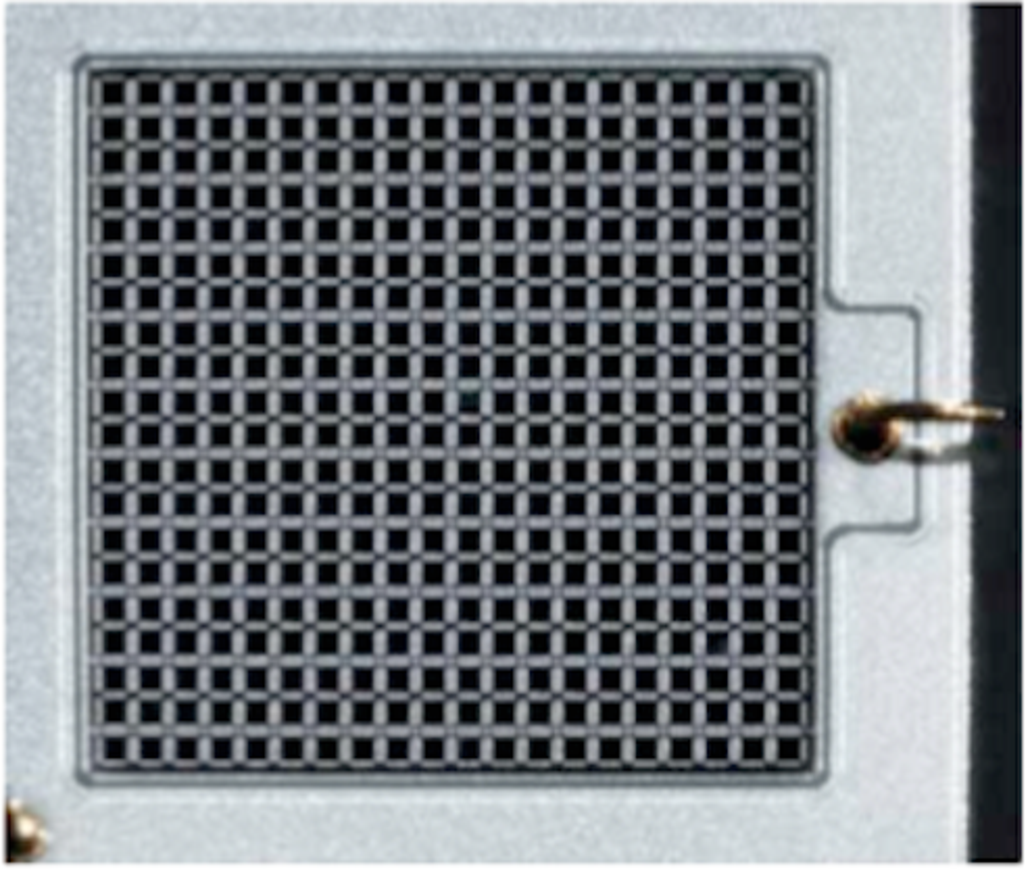
\includegraphics[height=0.22\textwidth]{PixelMatrix.pdf}}   
  \hspace{5mm}             
  \subfloat[\textit{Hamamatsu SiPM}]{%\label{fig:ad:ads7883}
  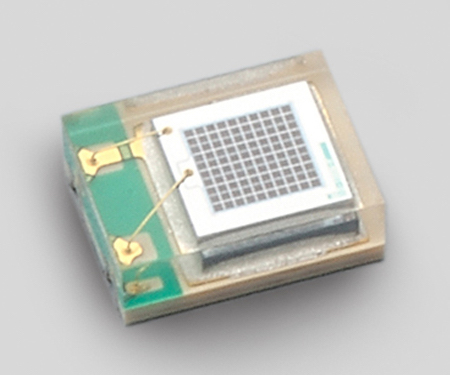
\includegraphics[height=0.22\textwidth]{sipm.jpg}}
  \hspace{5mm}             
  \subfloat[\textit{SiPM from SensL}]{%\label{fig:ad:ads7883}
  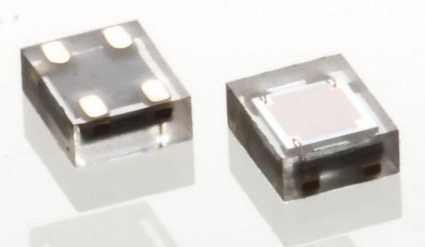
\includegraphics[height=0.22\textwidth]{sensl.jpg}}
  \caption{\textit{Silicon photomultipliers}}
  \label{fig:sipm}
\end{figure}

\section{KDB arrangement and cabling}
\label{sec:DB}

In this section we describe the KDB arrangement, in-vessel cabling and external cabling. A scheme of the cabling is shown if 
figure \ref{fig:cabling:scheme}). 

\begin{figure}[ht]
    \bigskip
    \begin{center}\leavevmode
        \rotatebox{0}{
        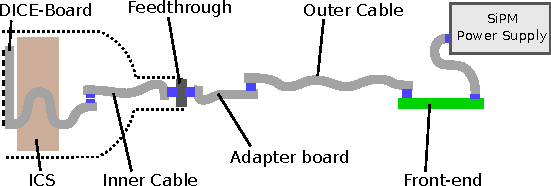
\includegraphics[width=.8\textwidth]{Simple.pdf}}
        \caption{\textit{Tracking plane cabling scheme.}}
        \label{fig:cabling:scheme}
    \end{center}
\end{figure}

\subsection*{Kapton DICE-Boards (KDBs) and in-vessel cabling}

The KDBs  where mounted on top of a thin plate of copper held by springs to the main copper plate that acts as a shielding. The reason of those springs is that they will allow for a small movement of the plate during the assembly and when closing the detector allowing for a perfect match of the tracking plane with the EL region. Fig. \ref{fig:spring_detail} shows the detail of one of those springs.

\begin{figure}[h!]
\begin{center}
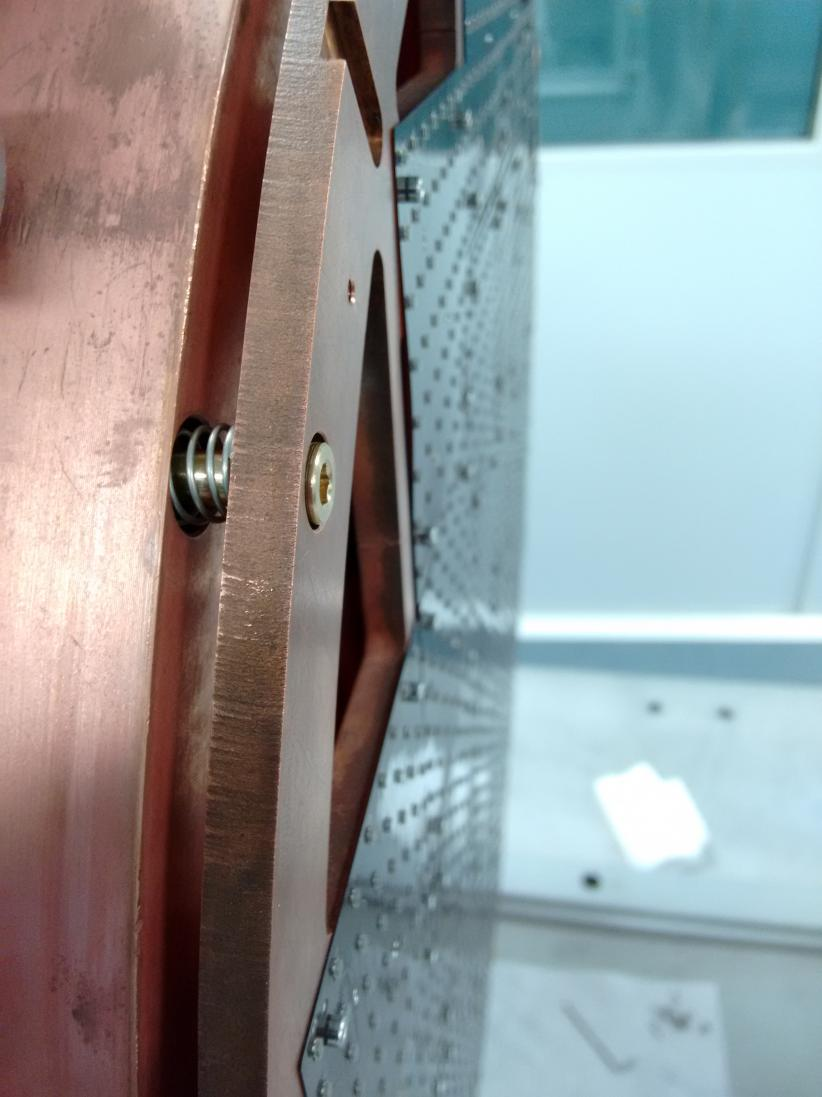
\includegraphics[width=0.45\textwidth]{IMG/spring_plate_detail}
%\hspace{15mm}
%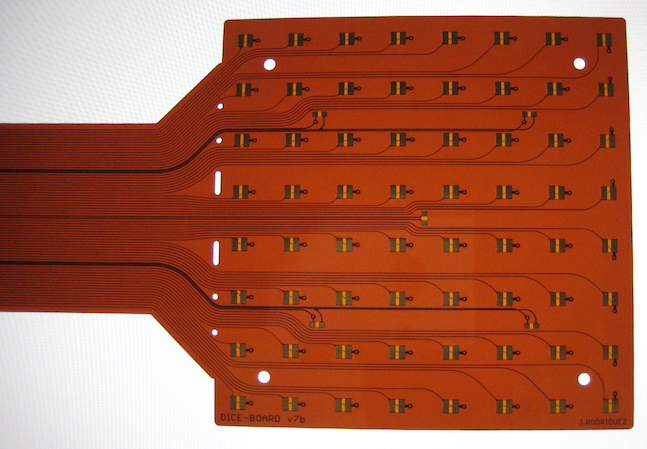
\includegraphics[width=0.39\textwidth]{IMG/DB.JPG}
\caption{Detail of one of the springs in the tracking plane thin plate that will allow to accomodate the tracking plane perfectly parallel to the electroluminescence region.}
\label{fig:spring_detail}
\end{center}
\end{figure}

Once the KDBs are mounted the tail has to be passed through the holes in the shielding plate (Fig. \ref{fig:cabling}). At the end of the tail a connector is soldered to plug a cable extension made of the same materials than the DICE-Boards. Those cables have to be organised to reach 5 different feed-throughs. The distribution of the cables is done using 3D printed structures placed inside a steel structure that will allow to extract the SiPMs cables and also is the point where the piping for vacuum and evacuation connects (Fig. \ref{fig:cabling_spaceship}).


\begin{figure}[h!]
\begin{center}
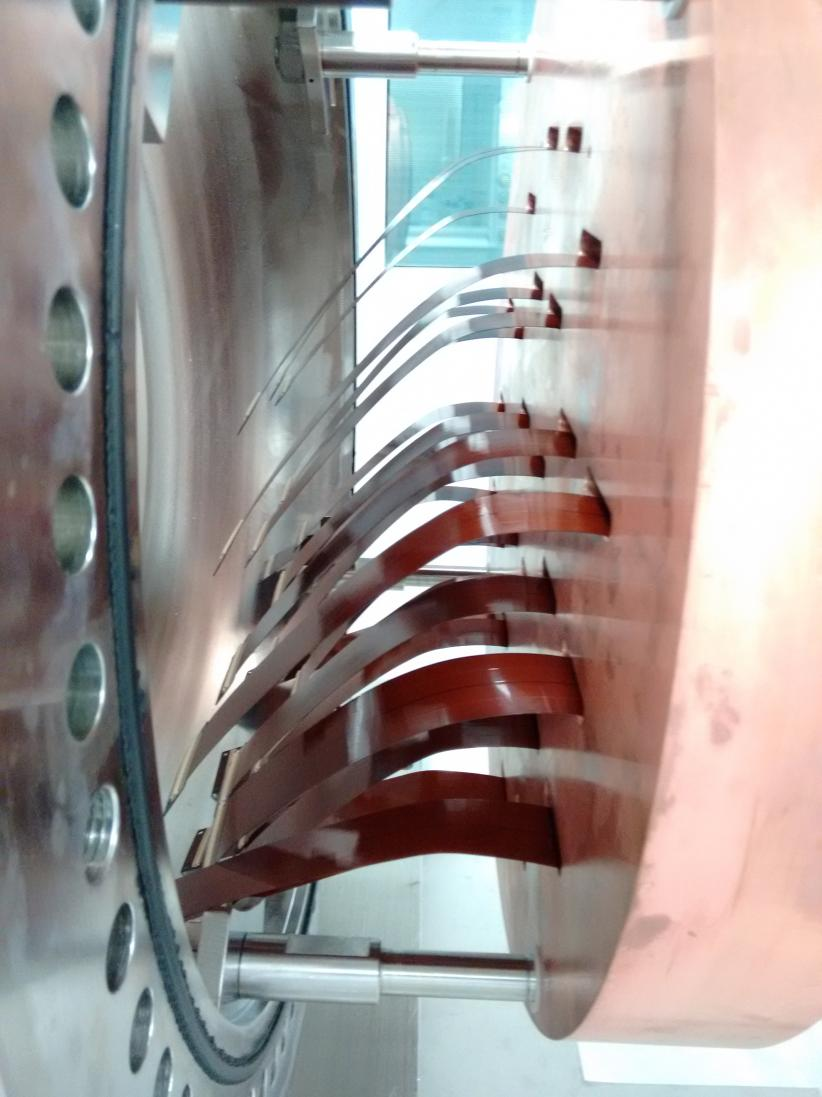
\includegraphics[width=0.45\textwidth]{IMG/cabling}
\caption{Dice-Boards cables passing through the holes in the shielding plate. At the end of the tail there is a connector that will allow for an extension of the cable to reach the feed-through.}
\label{fig:cabling}
\end{center}
\end{figure}

\begin{figure}[h!]
\begin{center}
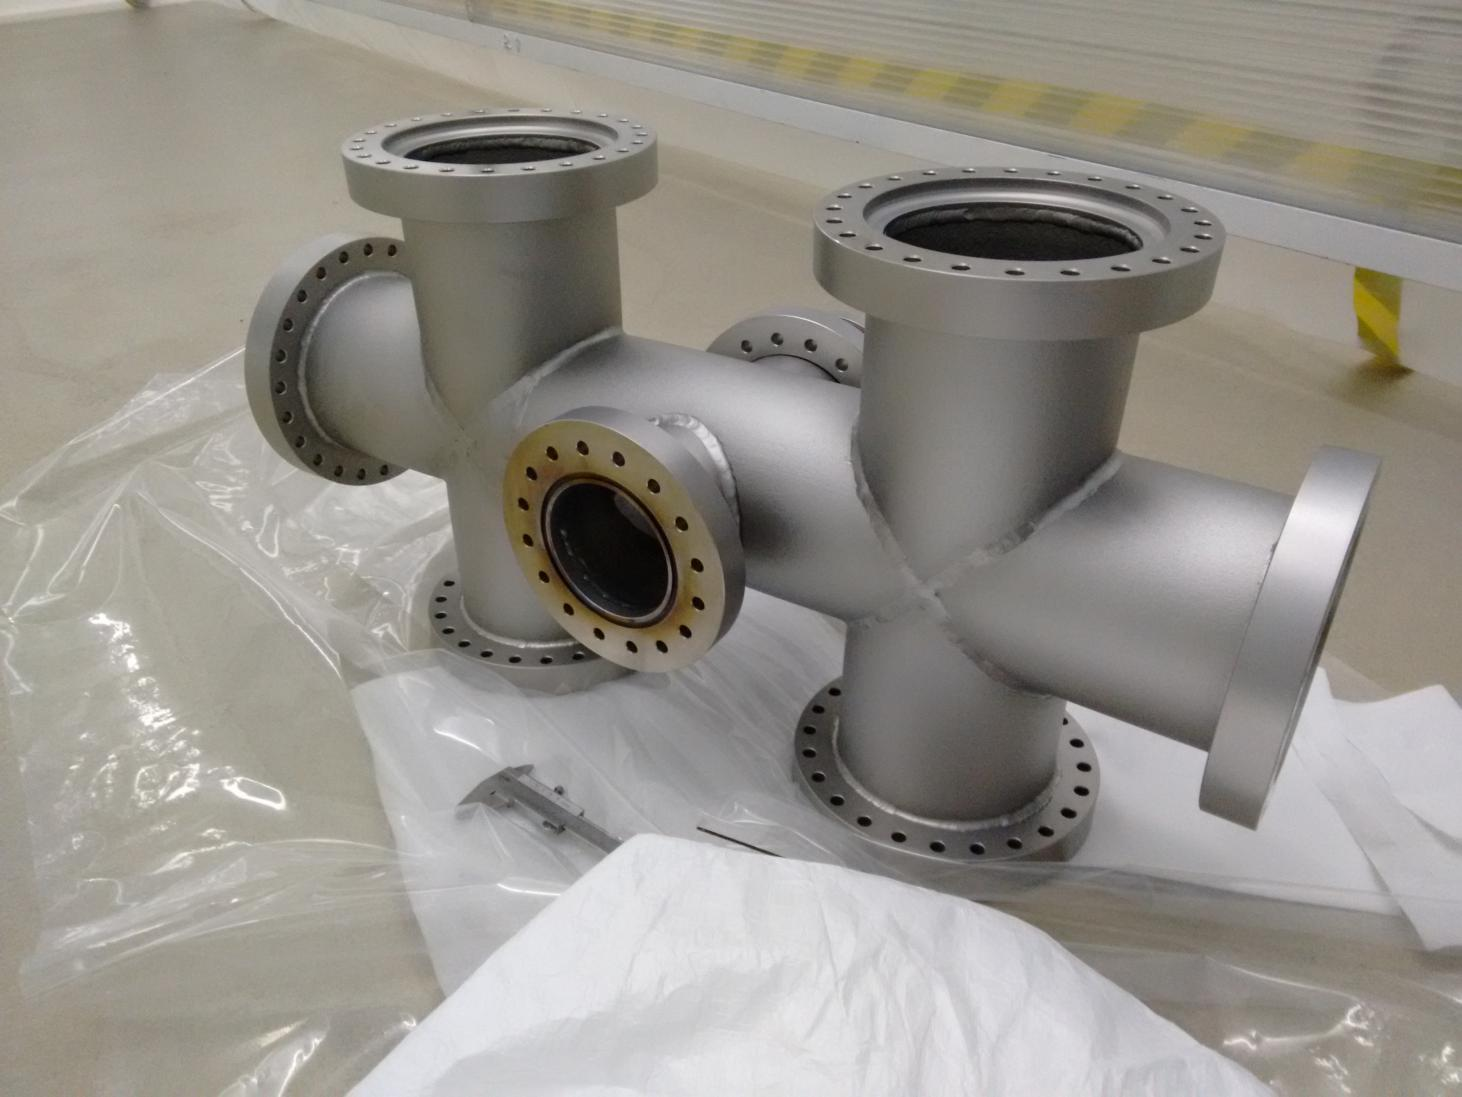
\includegraphics[width=0.45\textwidth]{IMG/spaceship_unmounted}
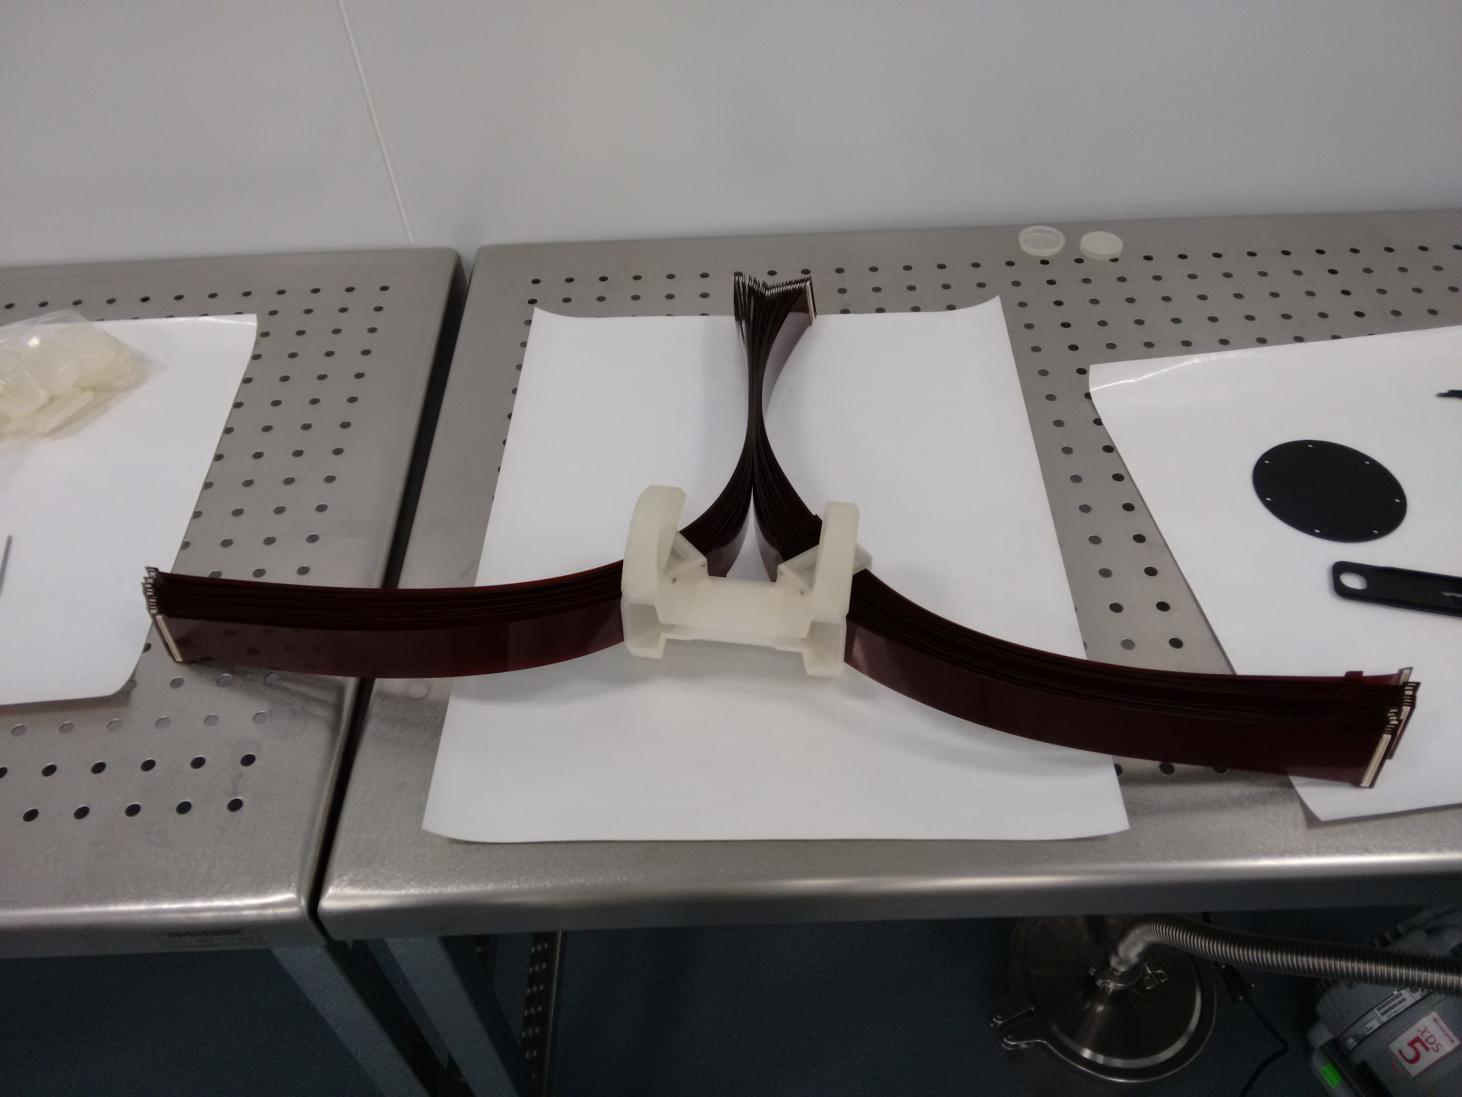
\includegraphics[width=0.45\textwidth]{IMG/spacechip_cabling}
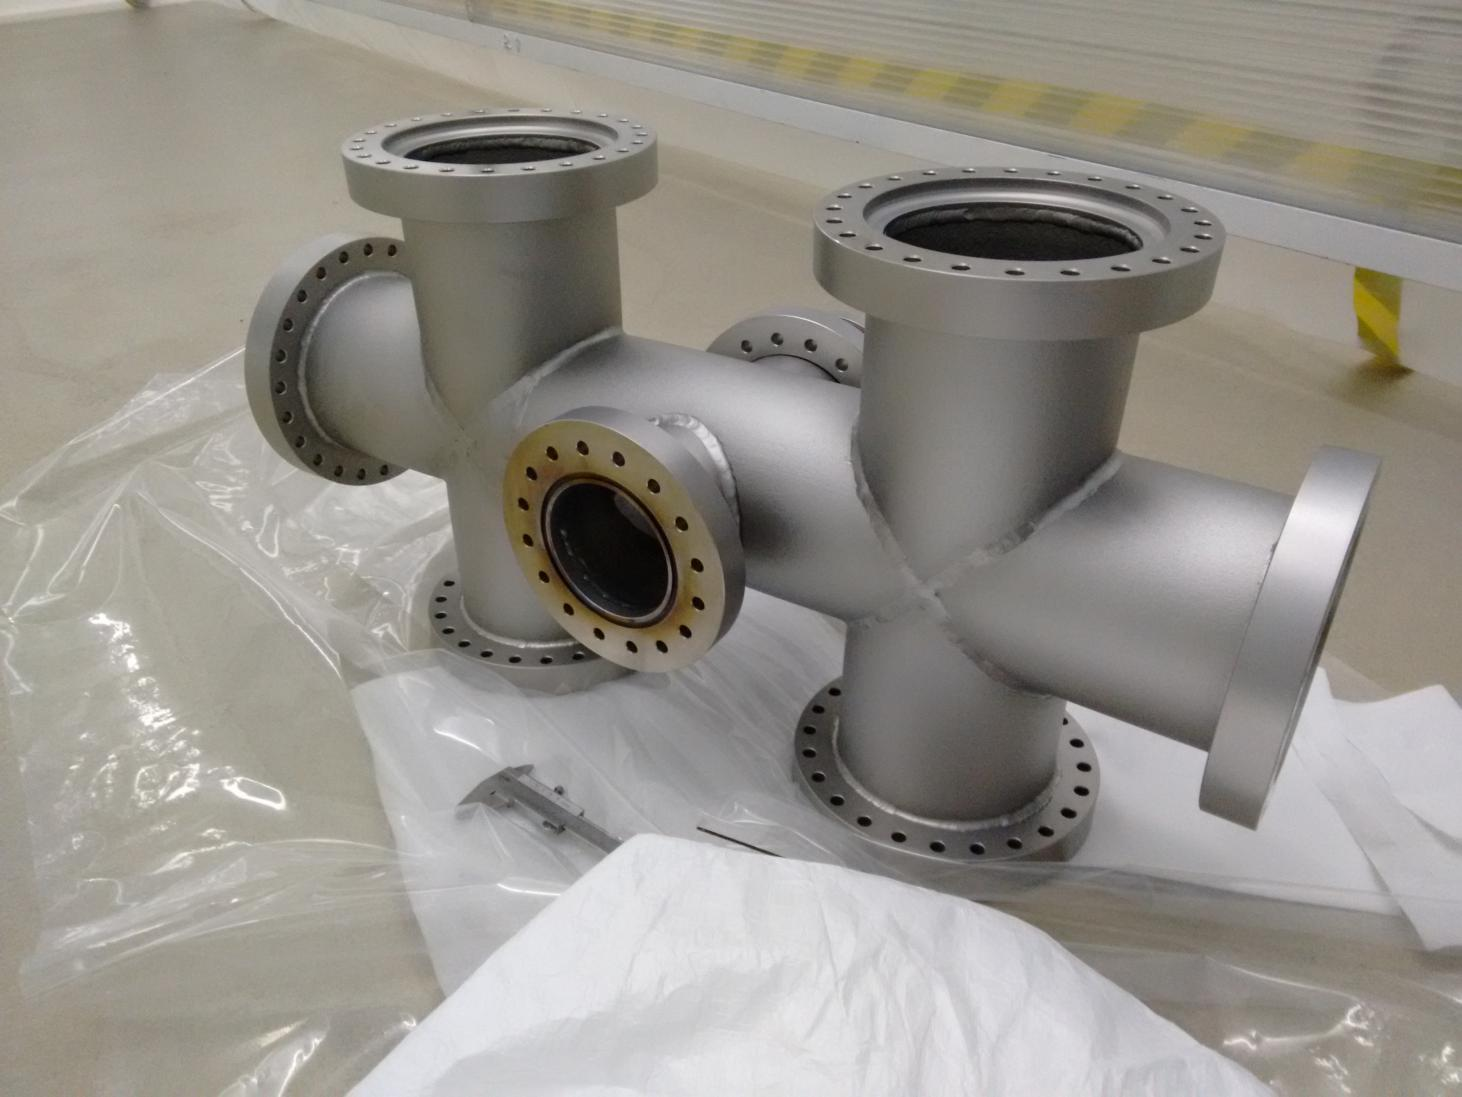
\includegraphics[width=0.45\textwidth]{IMG/spaceship_unmounted}
\caption{Up left: Steel structure to support and organize the SiPM cabling. Up right: 3D printed structure to allow a better distribution of the cables. Bottom: Assembly process of the SiPM cables.}
\label{fig:cabling_spaceship}
\end{center}
\end{figure}

The final step in the connection of inner cables of the tacking plane is the connexion to the tracking-plane feedthroughs (TPFT). Each one of these custom-made FTallows up to 6 KDB connexions. Extracting the signals of the 29 KDBs require then  5 TPFT. Figure \ref{fig:TPFT} shows the front and the back side of theTPFT as well as the cable connexion.

\begin{figure}[h!]
\centering
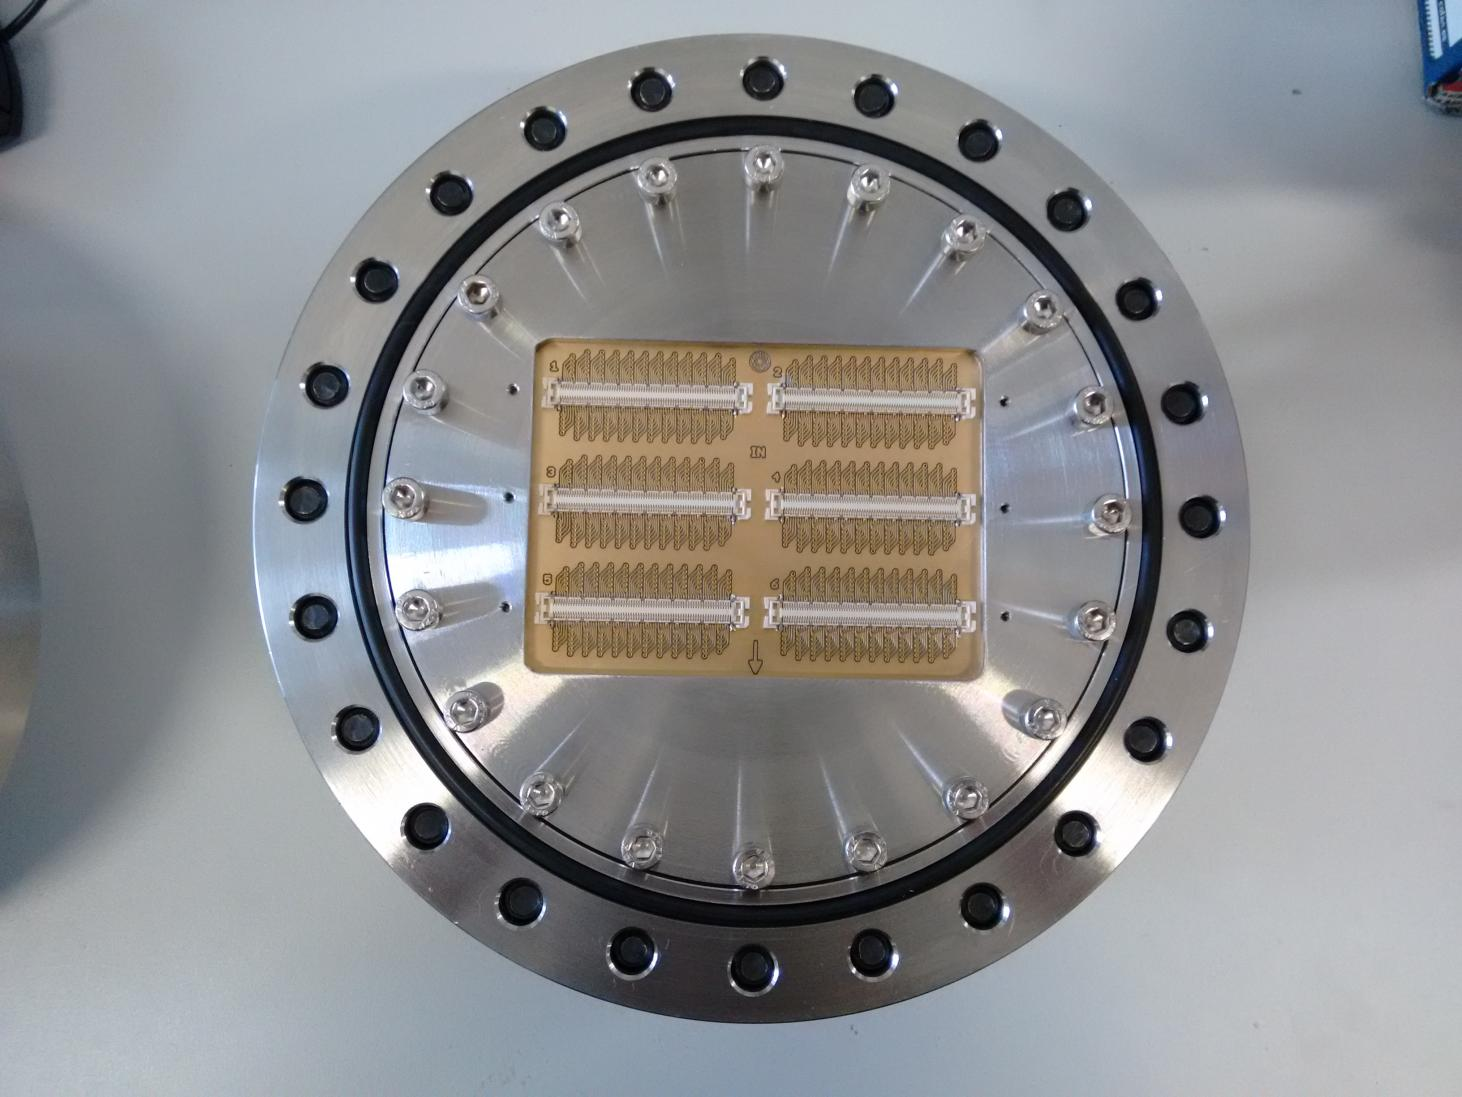
\includegraphics[width=0.45\textwidth]{IMG/TPFT1}
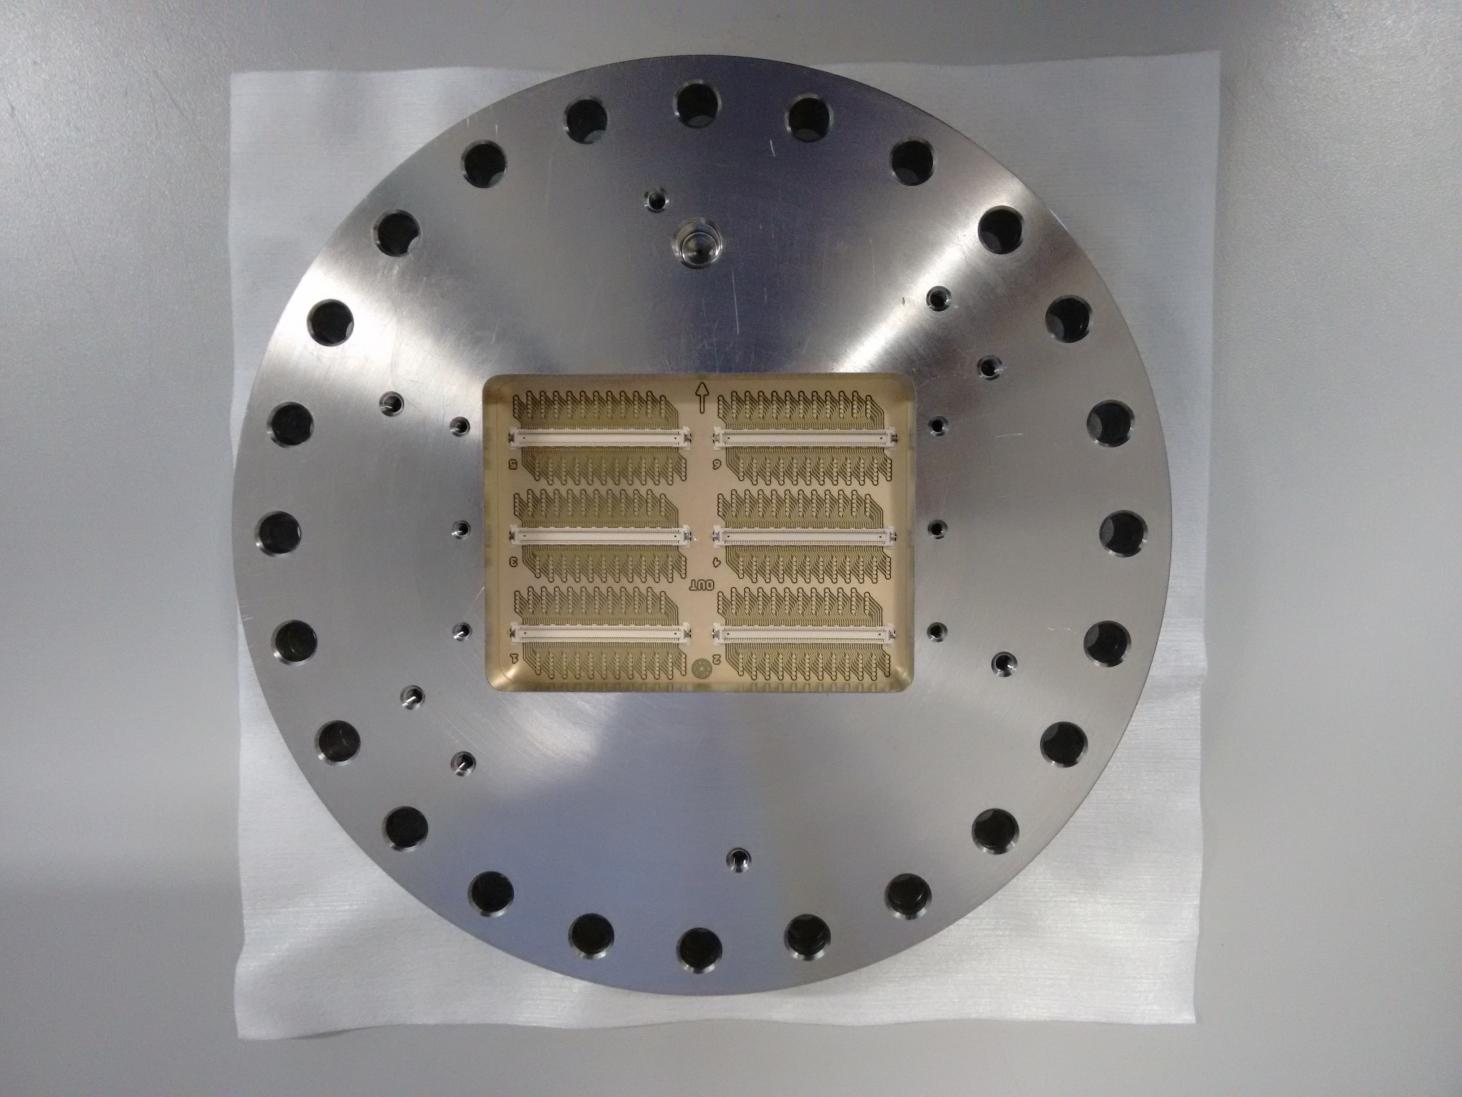
\includegraphics[width=0.45\textwidth]{IMG/TPFT2}
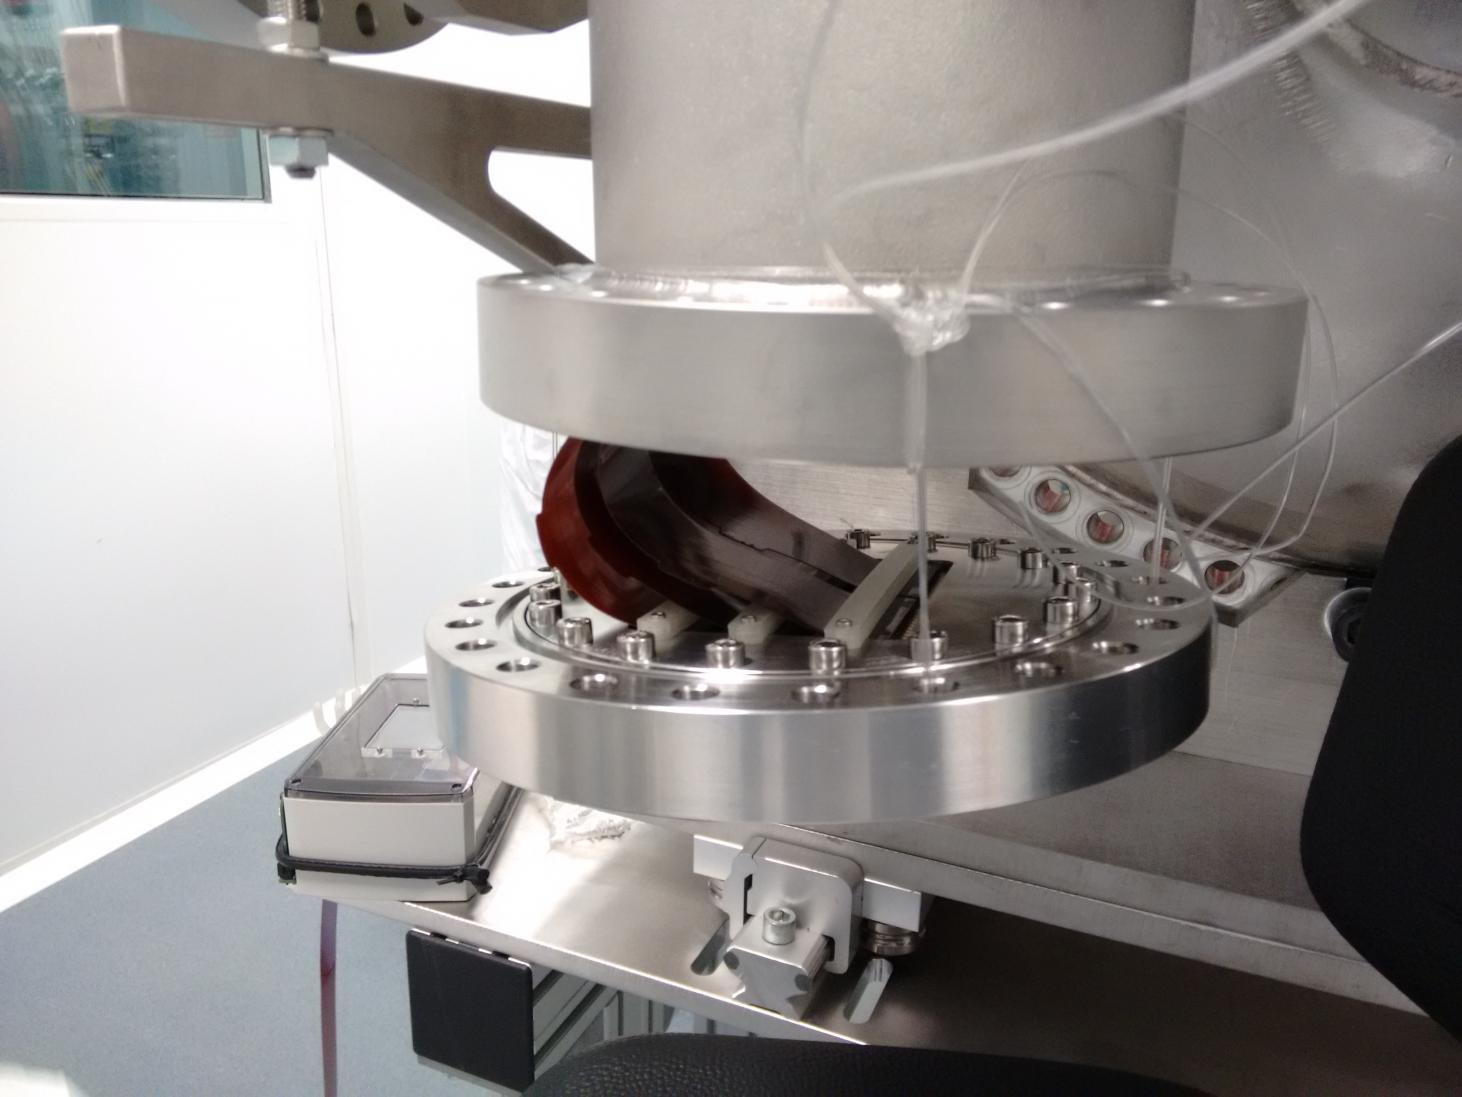
\includegraphics[width=0.45\textwidth]{IMG/TPFT_connected}
\caption{Up left: Inner side of the TPFT. Up right: external side of the TPFT. Bottom: Cable connexion.}
\label{fig:TPFT}
\end{figure}



\subsection{External cabling}\label{sec:ext}
In order to keep background events to a minimum, front-end electronics are placed nearby the detector but beyond the lead castle that surrounds the TPC, with a total cable length of $\sim$ 5 m from the sensor to the electronics. This poses a challenge in the design of a cabling solution that (1) is radio-clean enough to be inside the detector, (2) keeps enough signal-to-noise ratio in the relevant signal bandwidth for the gated integrator with a 5 m cable, (3) is cost-effective, (4) includes SiPM biasing voltage wires and (5) is also valid for the final NEXT phase (NEXT-100).

Differential transmission lines on fine-pitch FFC cables outside the detector were chosen as a good trade off between performance and cost. As shown in figure \ref{fig:external}, the cables are 0.5 mm pitch with $280 \times 76 \mu$m traces embedded in a thin polyester layer. The anode and the cathode of each SiPM are connected to the \textit{signal} and \textit{bias} lines respectively. Channels are separated by a guard trace connected to the analog ground in the front-end. Therefore three lines are needed for each SiPM channel. In addition, each KDB adds several more lines, for the  temperature sensor and  calibrating LEDs.

\begin{figure}[h!]
\centering
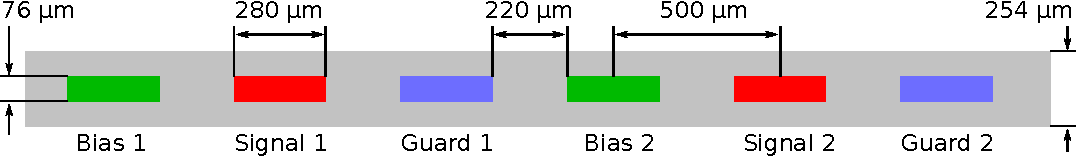
\includegraphics[width=.6\textwidth]{IMG/section.pdf}
\caption{Cross-section of the external cable (just two channels are shown).}
\label{fig:external}
\end{figure}

Since ommercial cables with the required density of traces were not available, the adopted solution was to split into four FFC cables. This way, the signals of a whole DICE-Board are distributed in four cables of 51 wires each. This distribution is done just at the output of the feedthrough, using a Kapton adapter board. This board has the same stackup as the DICE-Board or the inner cable, and splits the signals in four \textit{DF9 Hirose} connectors for the long cables.

In order to further reduce the noise coupled to the external cables, they are wrapped with a 1 mm aperture mesh, also connected to the analog ground at the front-end. This mesh is has its maximum attenuation rated at 1 MHz, which covers the range of frequencies we want to attenuate.

The external cables cables have been connected to the output of the TPFT and then they go below the platform until the position of the FEE boards where they are connected. (Fig. \ref{fig:external_installation})


\begin{figure}[h!]
\centering
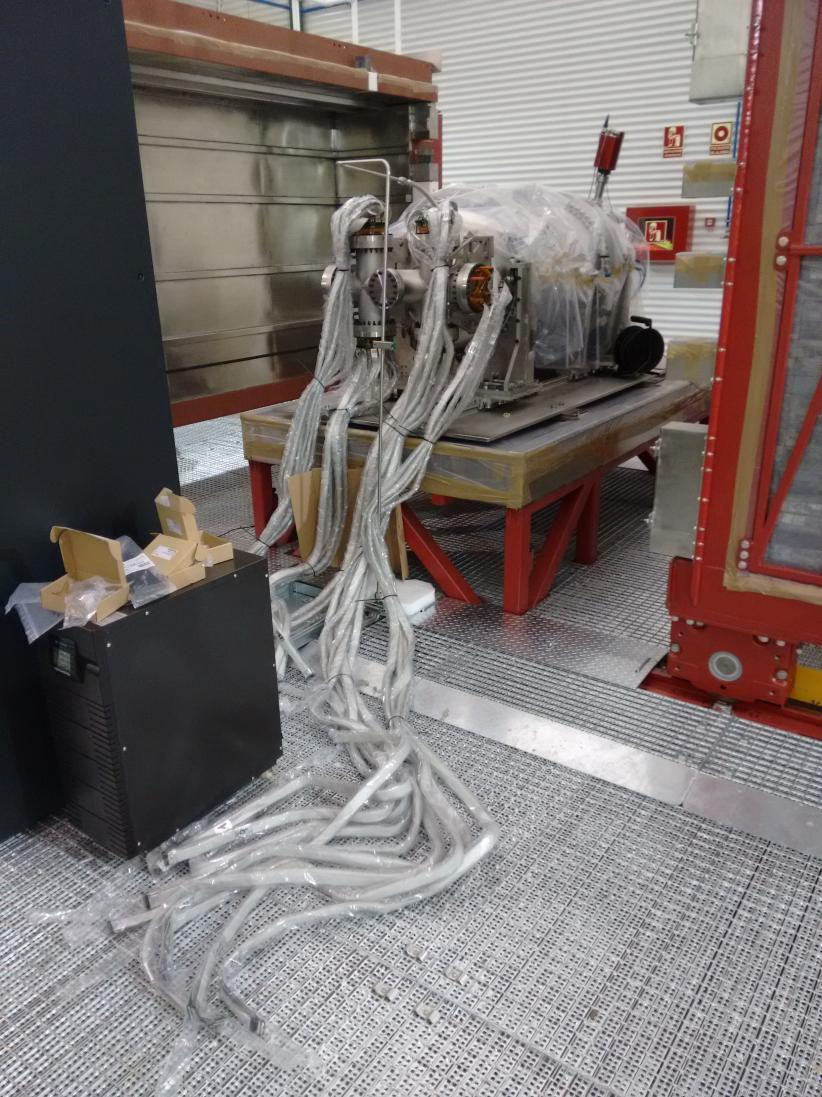
\includegraphics[width=.45\textwidth]{IMG/external_cabling2}
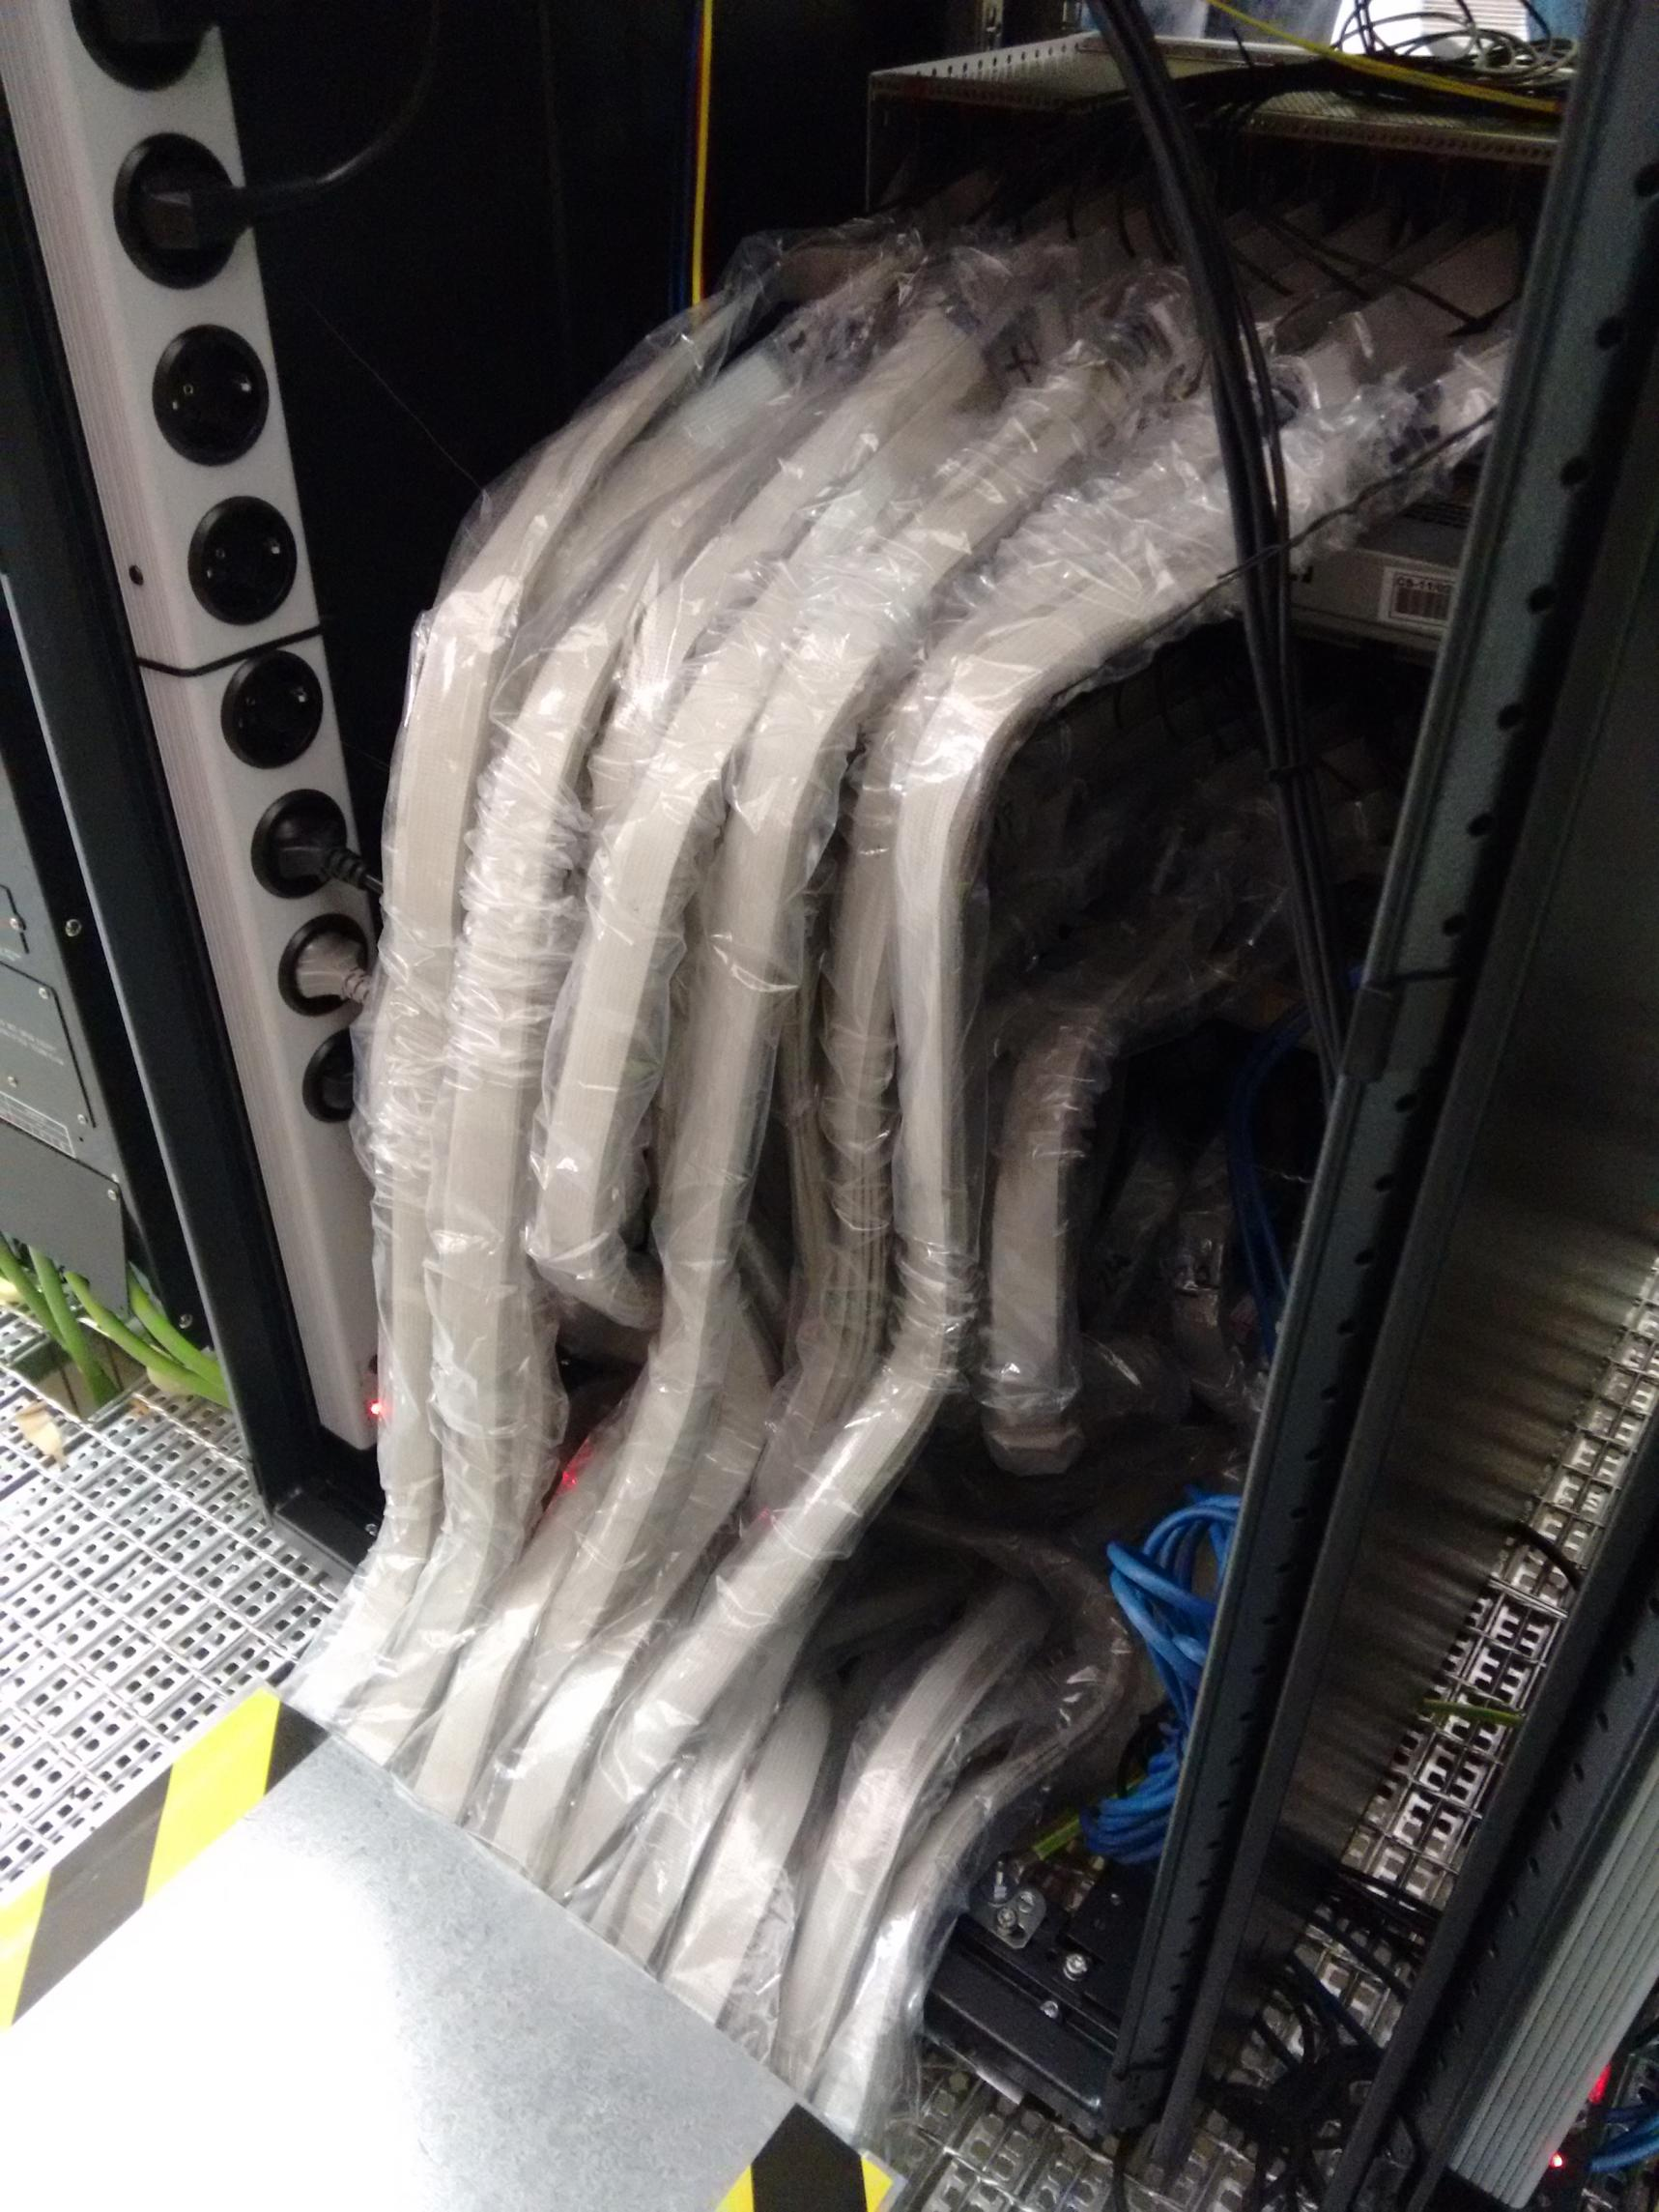
\includegraphics[width=.45\textwidth]{IMG/cabling2FEE}
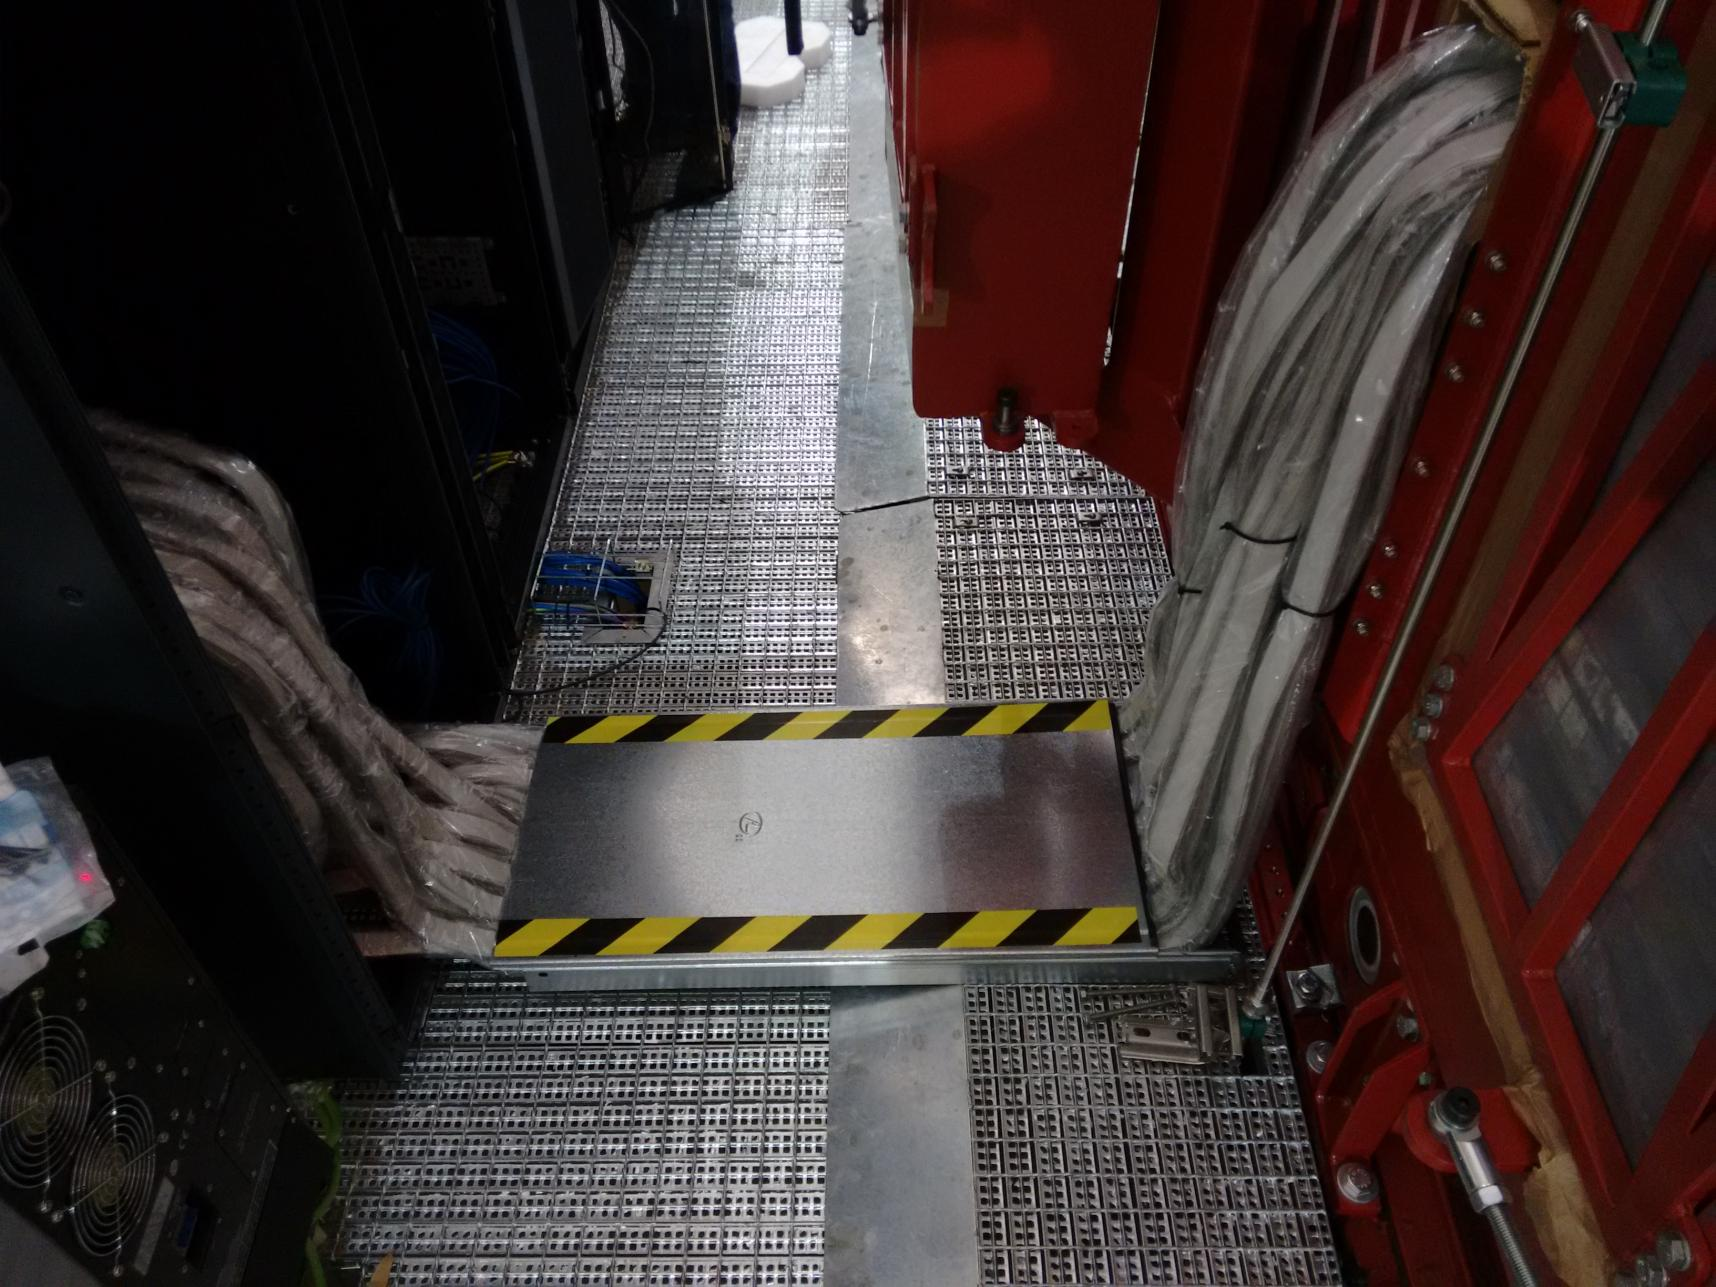
\includegraphics[width=.45\textwidth]{IMG/cabling_under_platform}
\caption{Different parts of the external cabling of the tracking plane. Up left shows a general view of the cabling. Up right picture is a detail of the connexion of the cables to the FEE boards. Bottom picture shows how the cables move under the platform.}
\label{fig:external_installation}
\end{figure}

\section{Sensor characterisaton}
The simplest method to calibrate the SiPMs is shown in figure \ref{fig:calibration} (top panel), and consists  in finding the different peaks associated to the different photoelectron numbers in the SiPM and extract the gain according to their separation. The first results from NEW show that the gain spread among the SiPMs is very small (figure \ref{fig:calibration} bottom).
%The first data extracted from the tracking plane has been used to make a first evaluation of the behaviour of the different sensors and DICE boards. The SiPMs have been tested with no light (only dark counts were recorded) and with light pulses from the blue LEDs installed in the energy plane (Fig. \ref{fig:calibration} bottom).

\begin{figure}[h!]
\centering
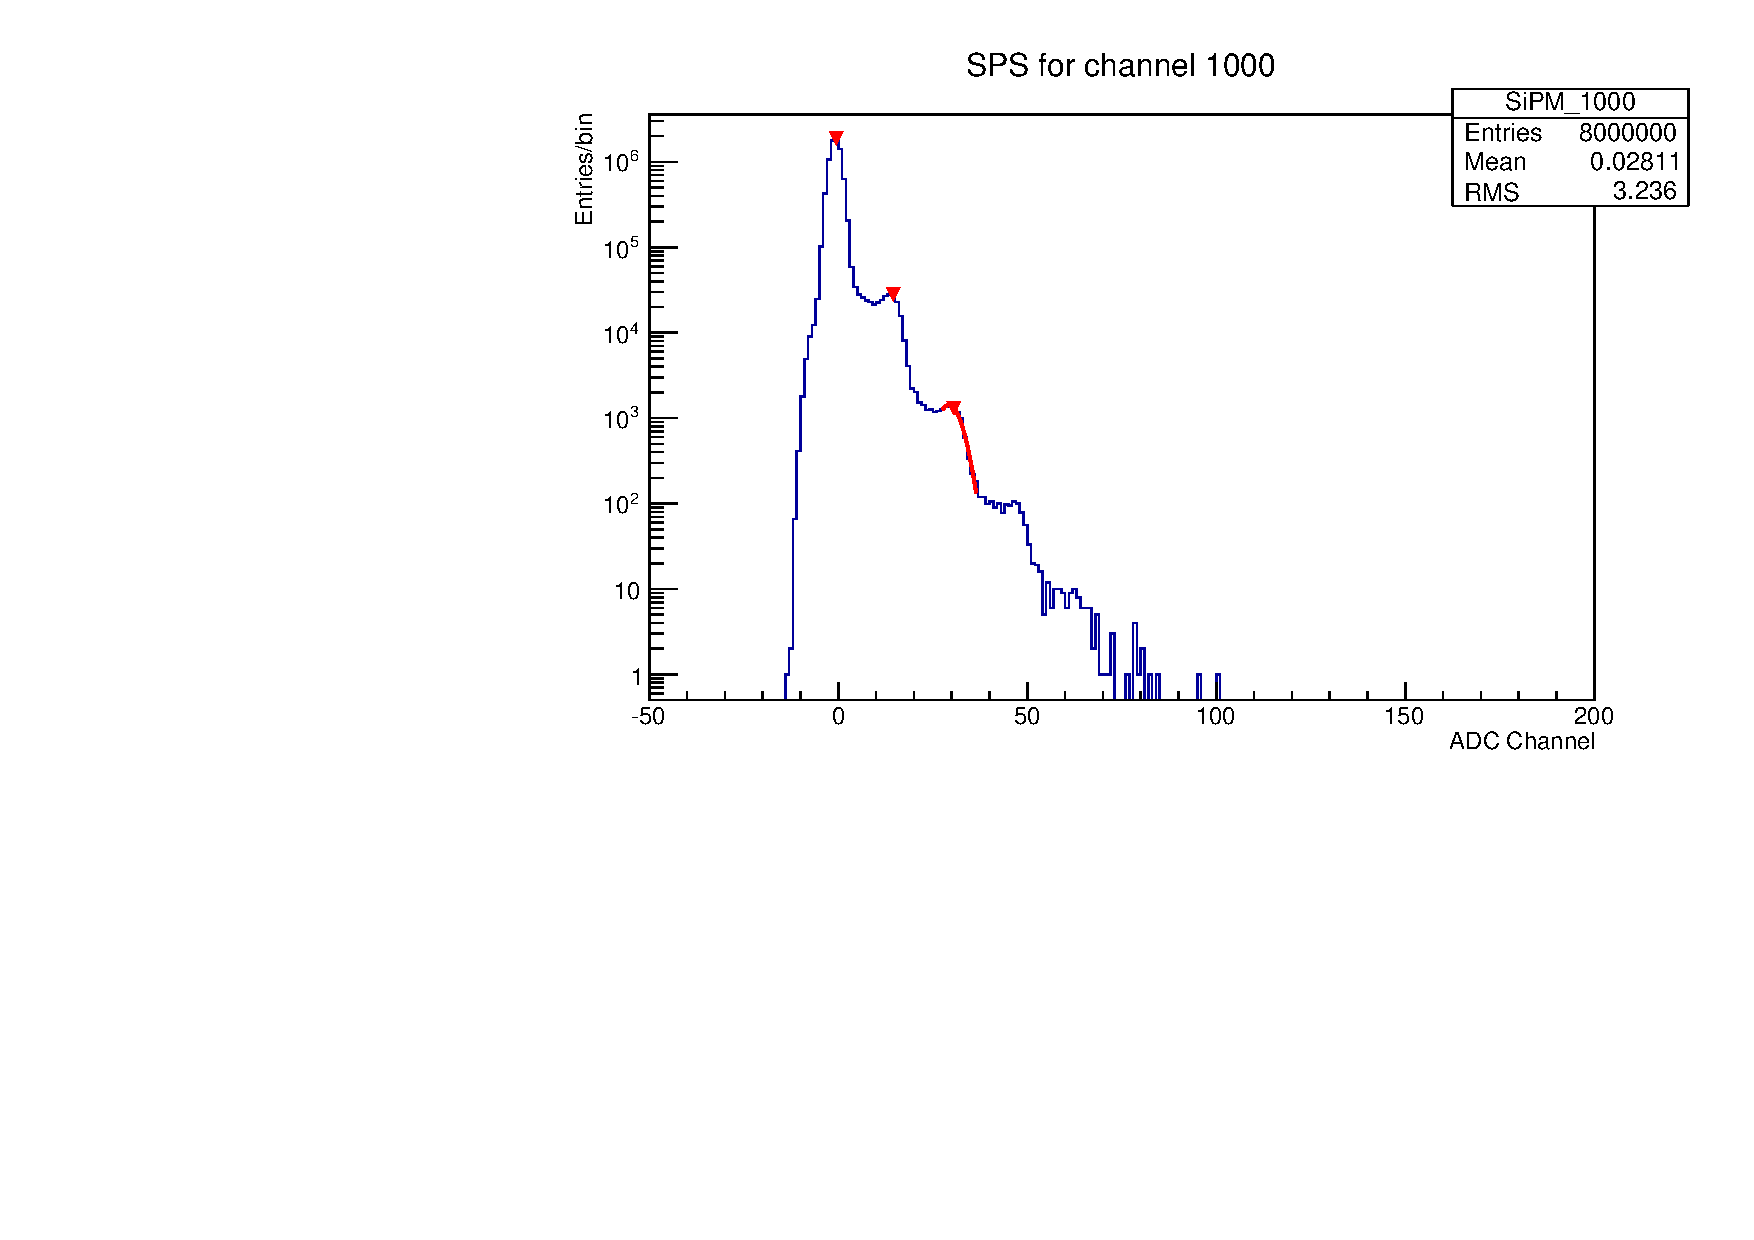
\includegraphics[width=0.45\textwidth]{IMG/normal_calibration}
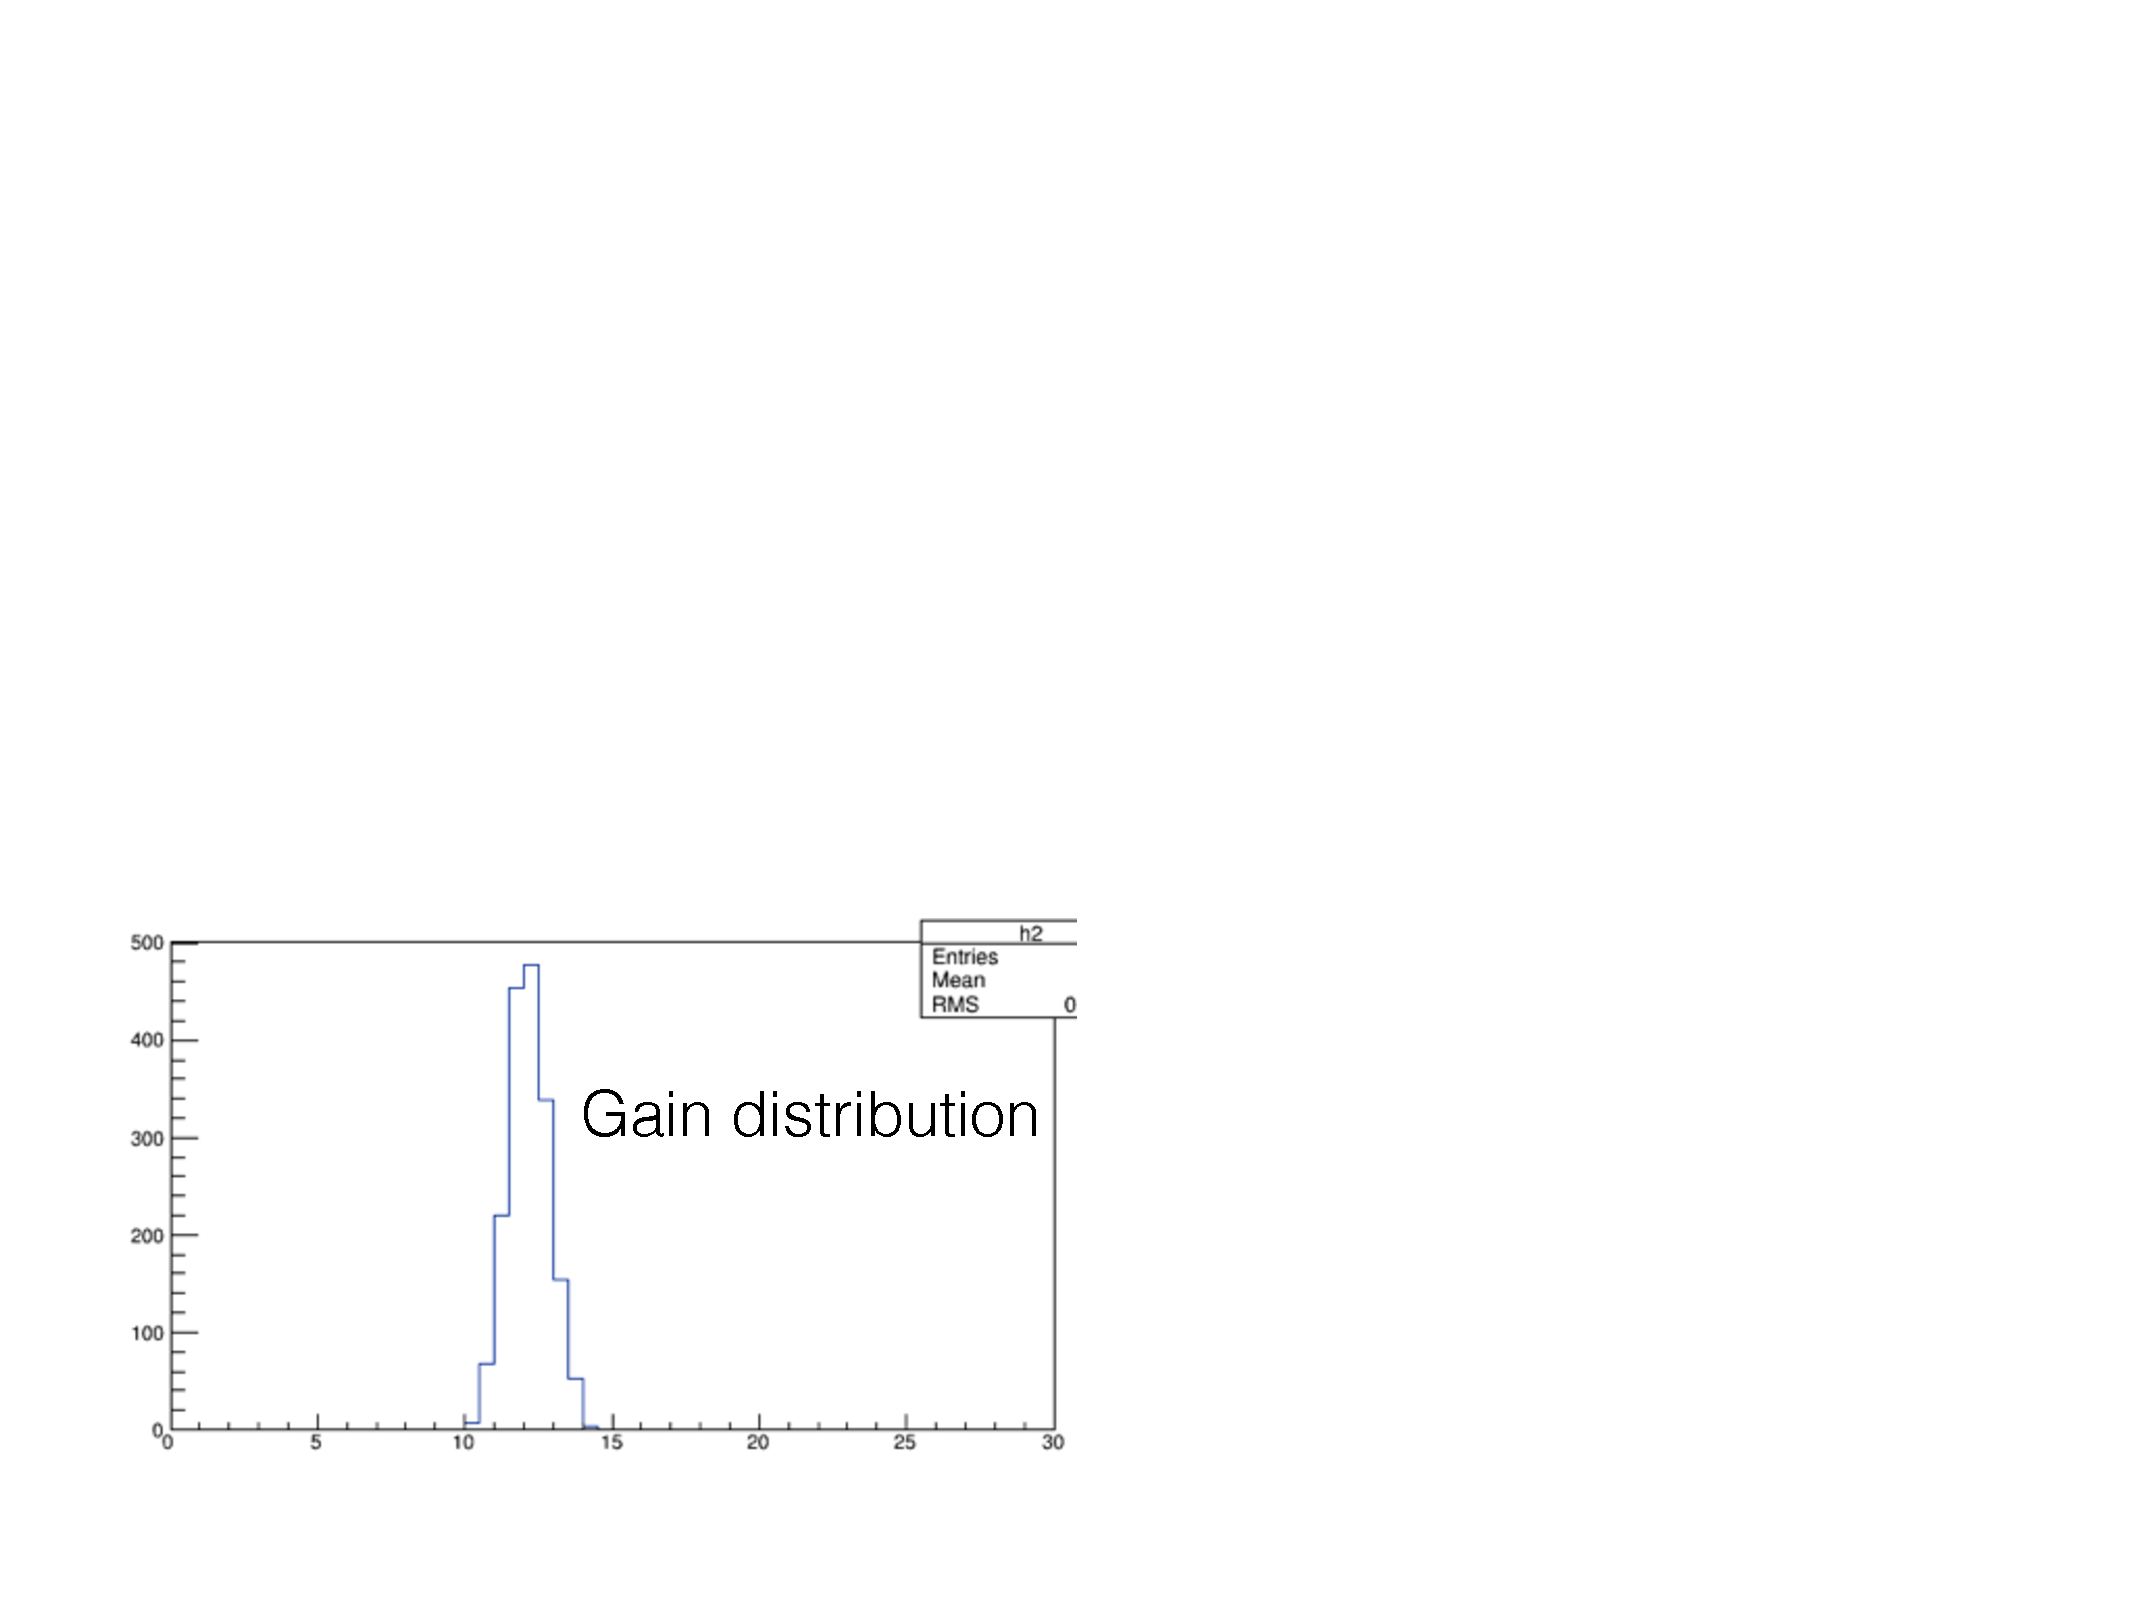
\includegraphics[width=0.45\textwidth]{IMG/SIPMsGain}
%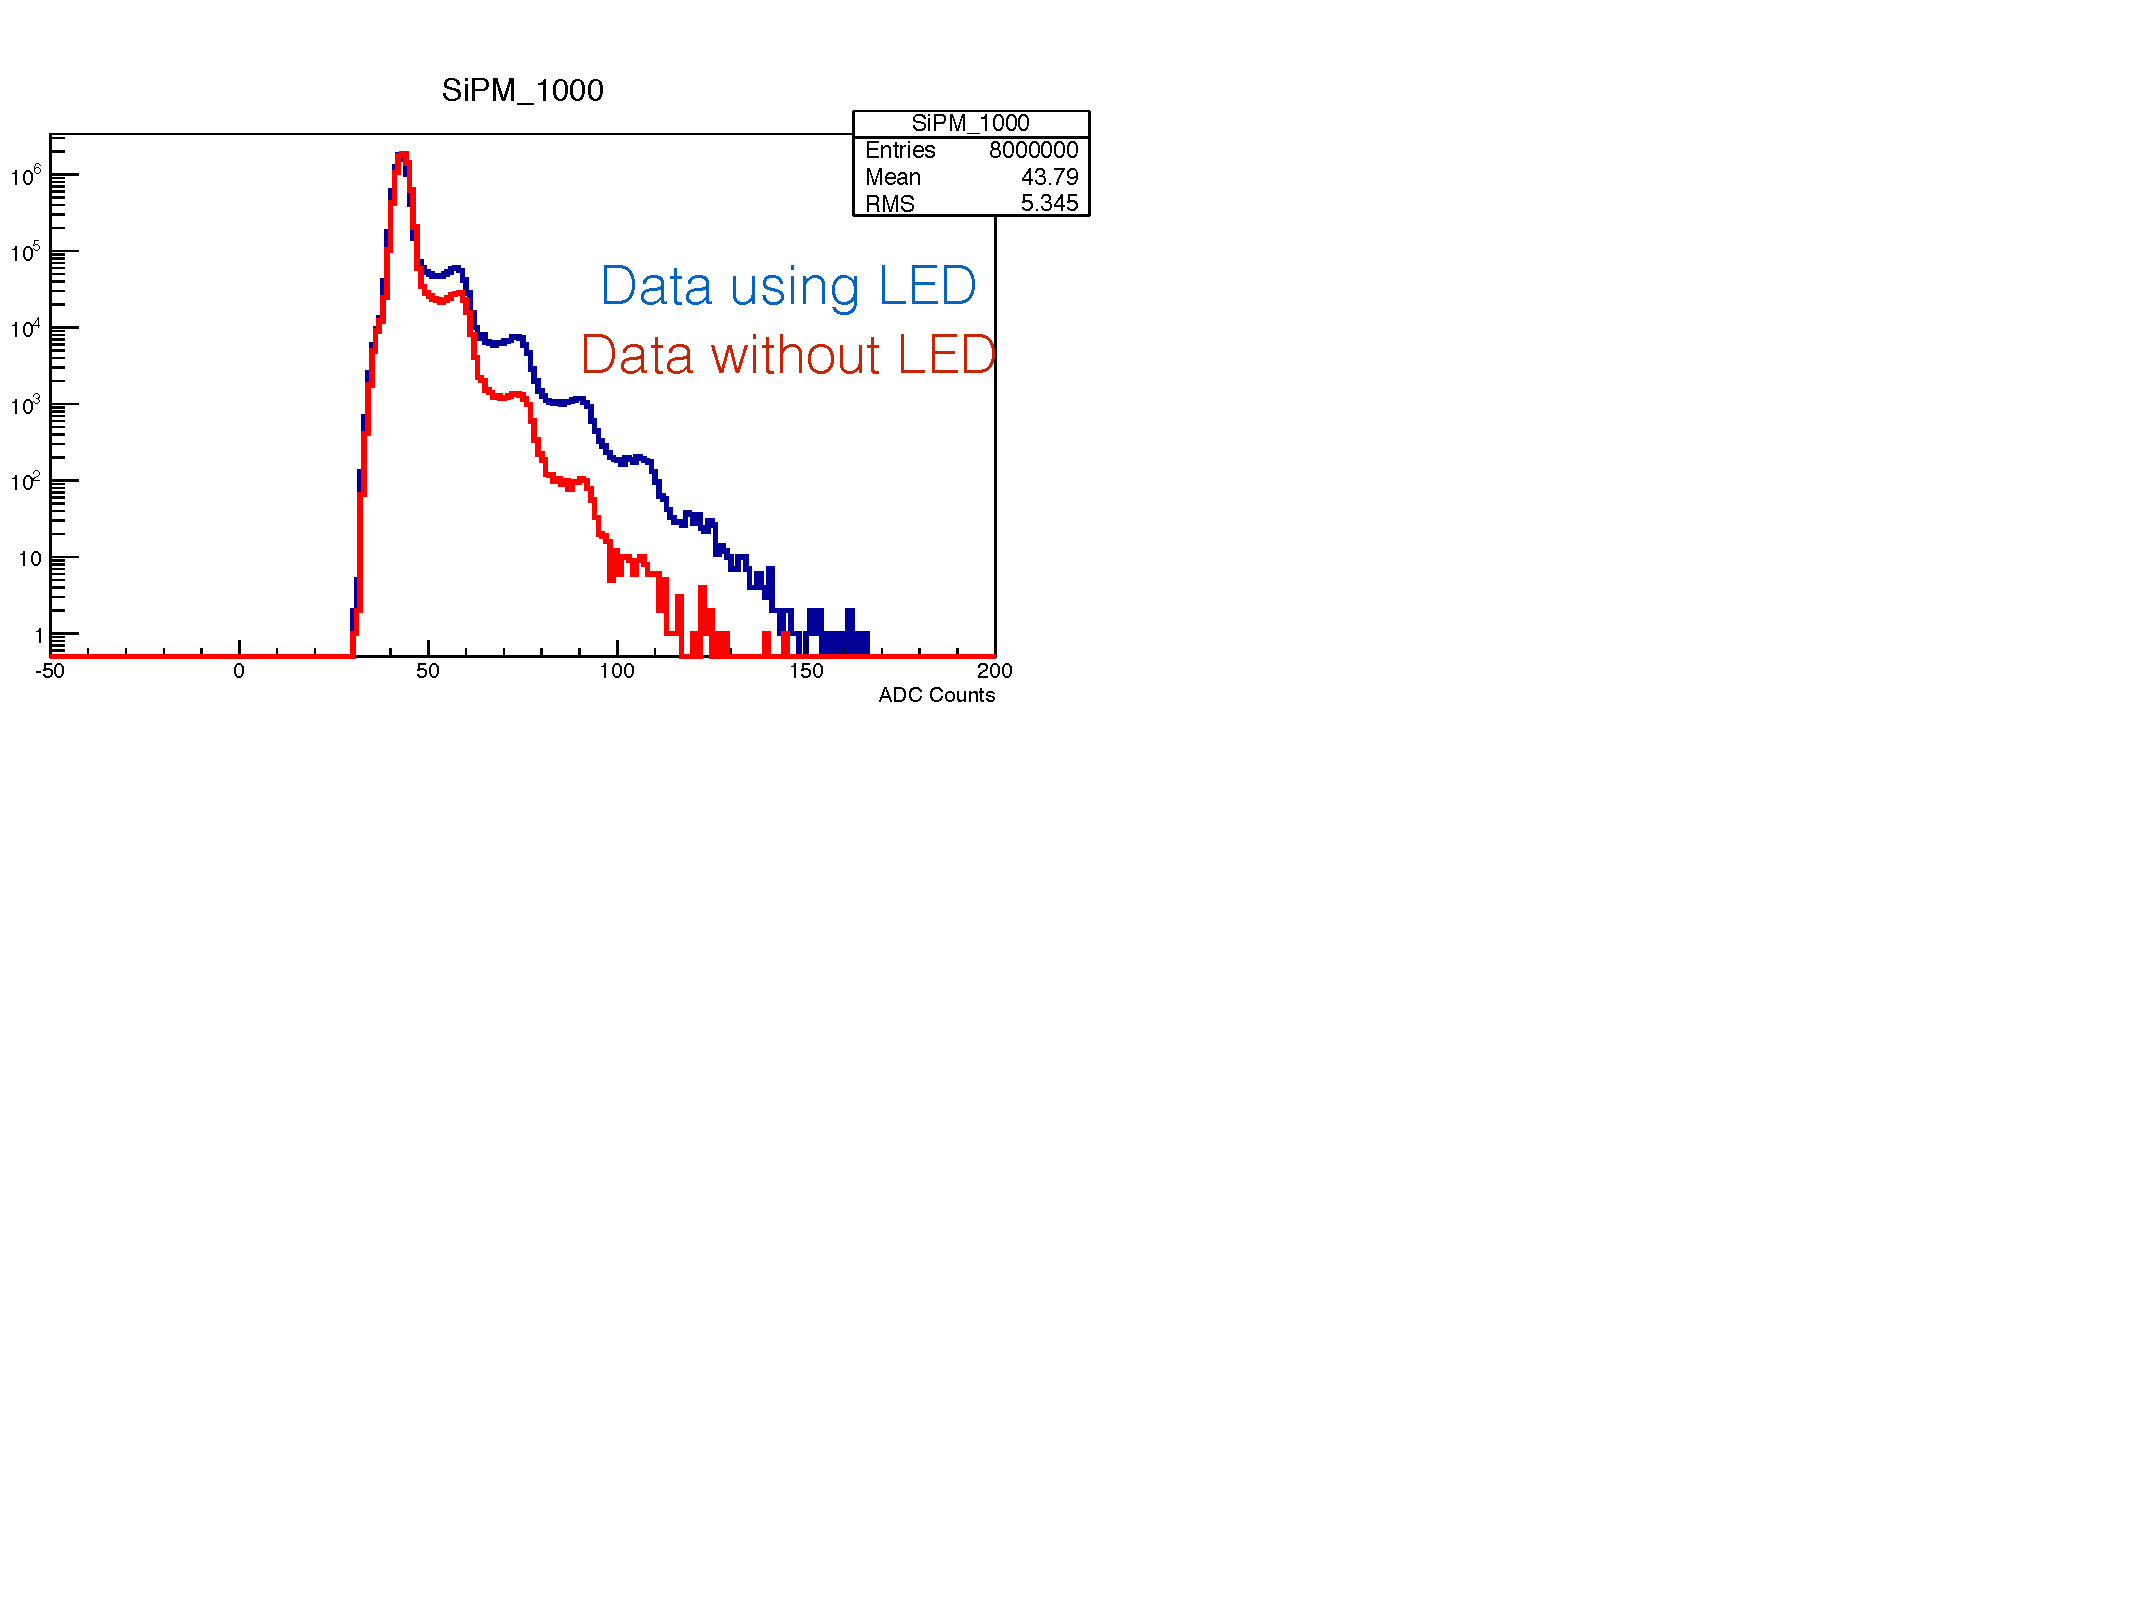
\includegraphics[width=0.45\textwidth]{IMG/SiPM_LED_noLED}
\caption{Top: standard method for calibration where the charge corresponding to the different number of photoelectrons in the SiPMs is estimated with a fit to the peak. The gain of the SiPM is calculated using the separation of the different peaks. Bottom: Histogram showing the gain of all the SiPMs in the plane. This histogram shows that the spread on the SiPMs gain is only of the order of a few ADC counts. 
%Bottom: Comparison of two spectra from the same SiPM, with (blue) and without light (red).
}
\label{fig:calibration}
\end{figure}

%Different methods for calibrating the SiPMs are currently being tested. The simplest method is based in a finding the different peaks associated to the different photoelectron number in the SiPM extract the gain according to their separation (Fig. \ref{fig:calibration} up left). This method was the one used in NEXT-DEMO and has demonstrated good performance. The first results show that the gain spread among the SiPMs is very small (Fig. \ref{fig:calibration} up right). However, some other methods may give a better characterization of the SiPMs that will include the integral effect of the dark count, quantum efficiency and cross-talk. Those other methods are being tested.
\section{Reflectors}

The material of choice for the KDBs (Kapton) as many advantages including flexibility, little degassing and radiopurity. However it is a poor reflector. In order to increase the amount of light recorded by the energy plane, a 2 mm teflon reflector is placed in front of each KDB. The reflectors (Fig. \ref{fig:reflector}) have holes to accommodate the SiPMs without damaging them and also have a space for the thermal sensor and the LEDs. However no holes are neccesary for the LEDs, since teflon is sufficiently transparent to the blue light they emit. 
\begin{figure}[h!]
\centering
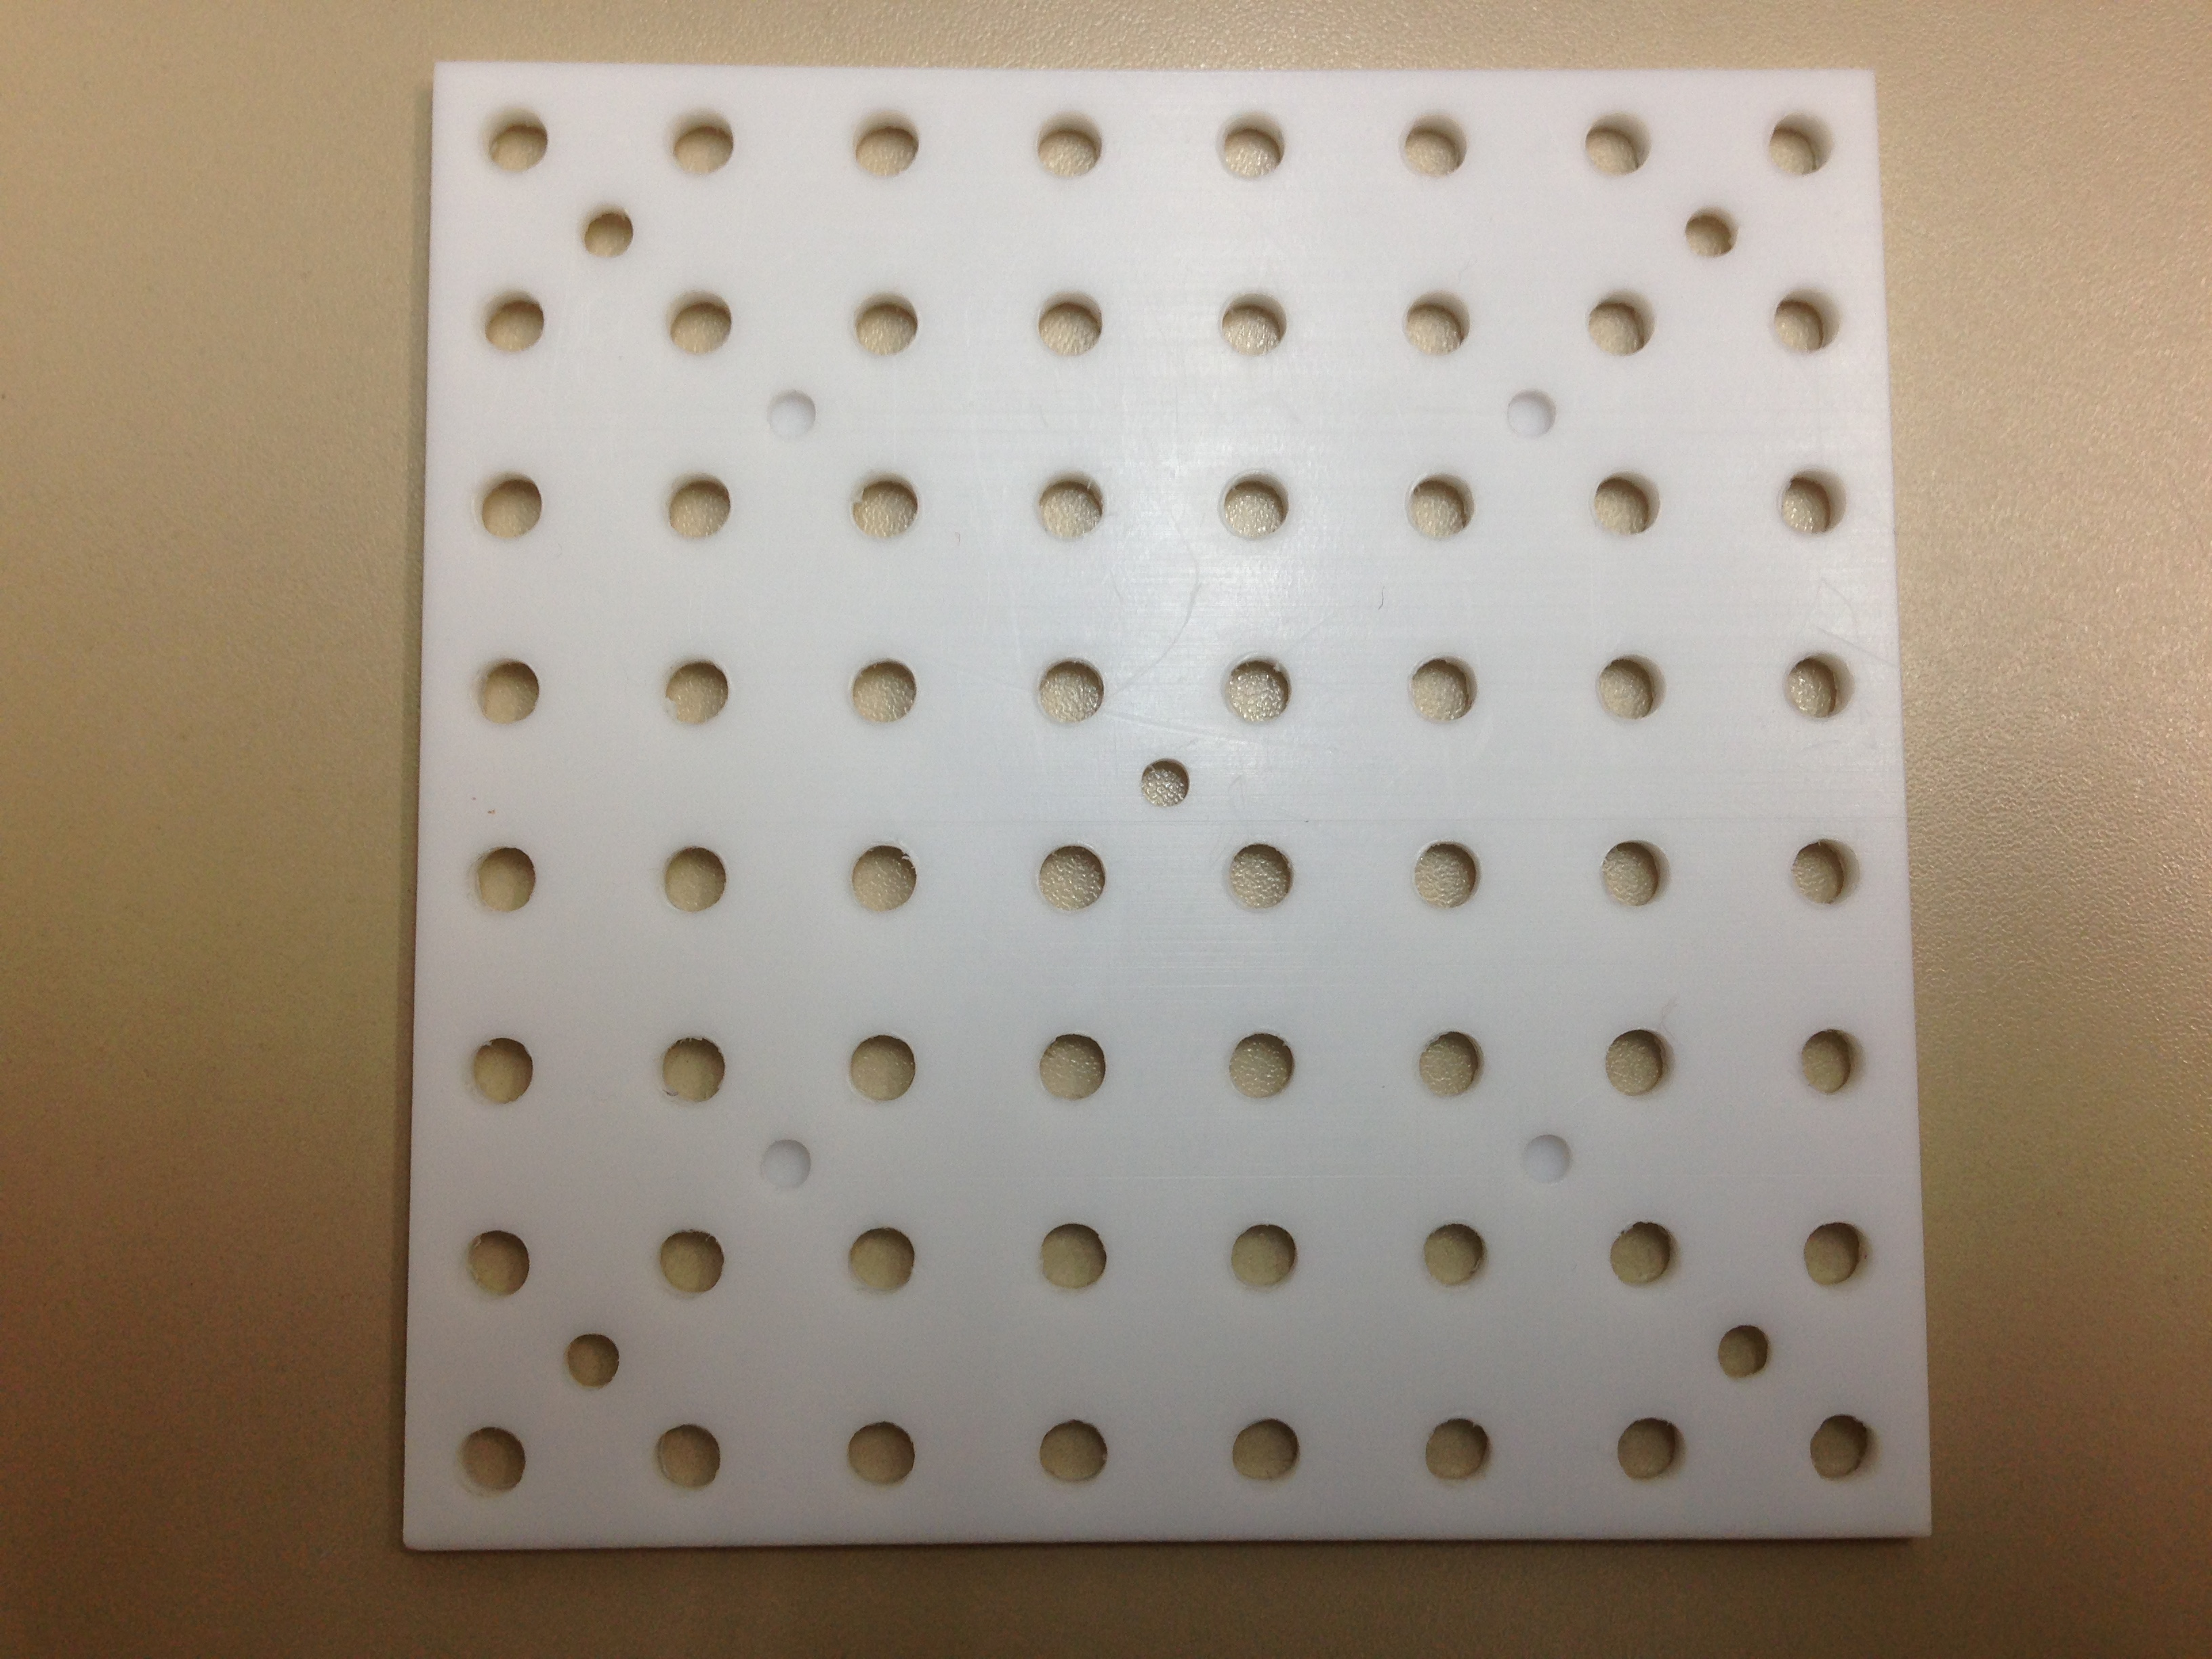
\includegraphics[width=0.45\textwidth]{IMG/teflon1}
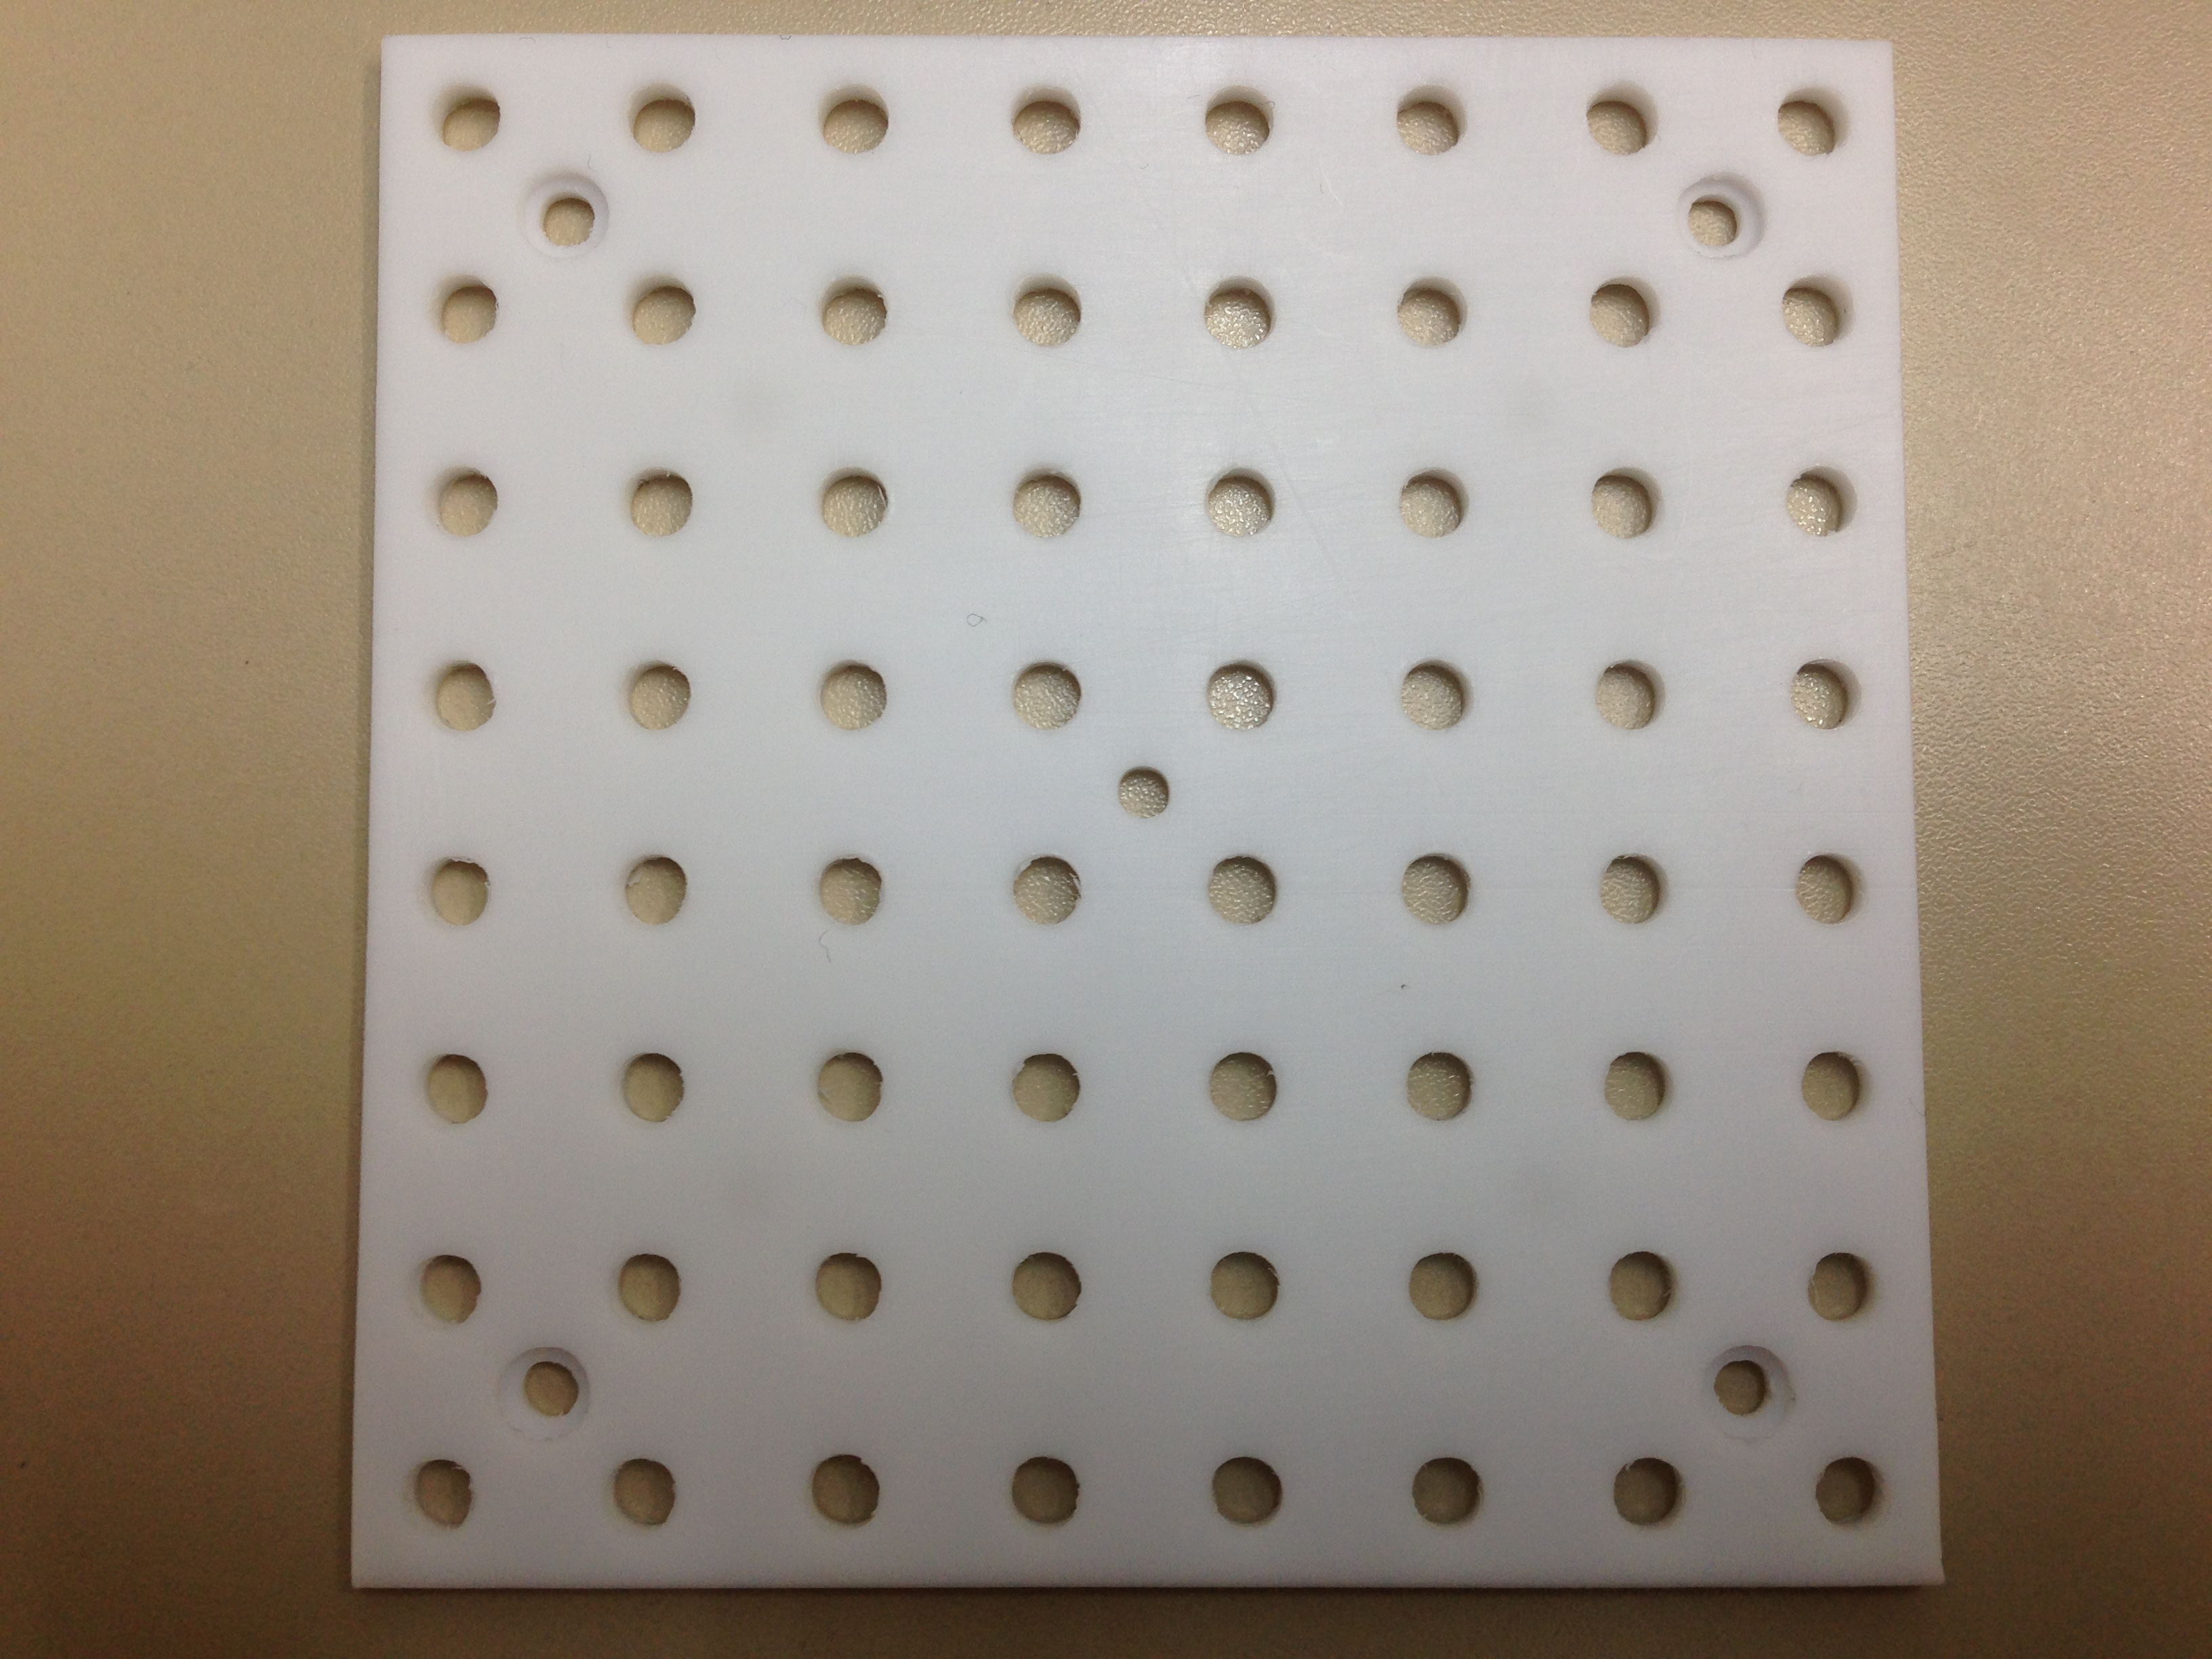
\includegraphics[width=0.45\textwidth]{IMG/teflon2}
\caption{Left: Back side (DB side) of the reflector. Right: Front side (EL) of the reflector.}
\label{fig:reflector}
\end{figure}


\section{Summary and status}

The main components of the tracking plane are installed and operational.



\newpage
\thispagestyle{empty}
\mbox{}

\bibitemsep = 3ex
\bibhang = 2em
\printbibliography[heading=bibintoc,title=Bibliography]

\end{document}




